\documentclass[twocolumn,astrosymb,twocolappendix]{aastex631}

%% The default is a single spaced, 10 point font, single spaced article.
%% There are 5 other style options available via an optional argument. They
%% can be invoked like this:
%%
%% \documentclass[arguments]{aastex631}
%% 
%% where the layout options are:
%%
%%  twocolumn   : two text columns, 10 point font, single spaced article.
%%                This is the most compact and represent the final published
%%                derived PDF copy of the accepted manuscript from the publisher
%%  manuscript  : one text column, 12 point font, double spaced article.
%%  preprint    : one text column, 12 point font, single spaced article.  
%%  preprint2   : two text columns, 12 point font, single spaced article.
%%  modern      : a stylish, single text column, 12 point font, article with
%% 		  wider left and right margins. This uses the Daniel
%% 		  Foreman-Mackey and David Hogg design.
%%  RNAAS       : Supresses an abstract. Originally for RNAAS manuscripts 
%%                but now that abstracts are required this is obsolete for
%%                AAS Journals. Authors might need it for other reasons. DO NOT
%%                use \begin{abstract} and \end{abstract} with this style.
%%
%% Note that you can submit to the AAS Journals in any of these 6 styles.
%%
%% There are other optional arguments one can invoke to allow other stylistic
%% actions. The available options are:
%%
%%   astrosymb    : Loads Astrosymb font and define \astrocommands. 
%%   tighten      : Makes baselineskip slightly smaller, only works with 
%%                  the twocolumn substyle.
%%   times        : uses times font instead of the default
%%   linenumbers  : turn on lineno package.
%%   trackchanges : required to see the revision mark up and print its output
%%   longauthor   : Do not use the more compressed footnote style (default) for 
%%                  the author/collaboration/affiliations. Instead print all
%%                  affiliation information after each name. Creates a much 
%%                  longer author list but may be desirable for short 
%%                  author papers.
%% twocolappendix : make 2 column appendix.
%%   anonymous    : Do not show the authors, affiliations and acknowledgments 
%%                  for dual anonymous review.
%%
%% these can be used in any combination, e.g.
%%
%% \documentclass[twocolumn,linenumbers,trackchanges]{aastex631}
%%
%% AASTeX v6.* now includes \hyperref support. While we have built in specific
%% defaults into the classfile you can manually override them with the
%% \hypersetup command. For example,
%%
%% \hypersetup{linkcolor=red,citecolor=green,filecolor=cyan,urlcolor=magenta}
%%
%% will change the color of the internal links to red, the links to the
%% bibliography to green, the file links to cyan, and the external links to
%% magenta. Additional information on \hyperref options can be found here:
%% https://www.tug.org/applications/hyperref/manual.html#x1-40003
%%
%% Note that in v6.3 "bookmarks" has been changed to "true" in hyperref
%% to improve the accessibility of the compiled pdf file.
%%
%% If you want to create your own macros, you can do so
%% using \newcommand. Your macros should appear before
%% the \begin{document} command.
%%
\newcommand{\vdag}{(v)^\dagger}
\newcommand\aastex{AAS\TeX}
\newcommand\latex{La\TeX}
% \newcommand{\sbunit}{mag~arcsec$^{-2}$}
\newcommand{\sbunit}{\mathrm{mag\ arcsec}^{-2}}
\newcommand{\sbcen}{\mu_{0}(g)}
\newcommand{\sbeff}{\overline{\mu}_{\mathrm{eff}}(g)}
\newcommand{\sbeffr}{\overline{\mu}_{\mathrm{eff}}(r)}
\newcommand{\jiaxuan}[1]{\textcolor{orange}{\textbf{Jiaxuan: #1}}}


% \newcommand{\code}[1]{\textbf{\texttt{#1}}}
\newcommand{\code}[1]{\texttt{#1}}
\newcommand{\sersic}{S\'ersic}
\usepackage{CJKutf8}
\usepackage{bm}
\usepackage{appendix}
\usepackage{amsmath,amssymb}

%% Reintroduced the \received and \accepted commands from AASTeX v5.2
% \received{\today}
% \revised{\today}
% \accepted{\today}

% \submitjournal{ApJ}

%% alias for citations
\defcitealias{Greco2018}{G18}

\shorttitle{UDGs in MW analogs}
\shortauthors{Li et al.}
%%
%% You can add a light gray and diagonal water-mark to the first page 
%% with this command:
%% \watermark{text}
%% where "text", e.g. DRAFT, is the text to appear.  If the text is 
%% long you can control the water-mark size with:
%% \setwatermarkfontsize{dimension}
%% where dimension is any recognized LaTeX dimension, e.g. pt, in, etc.
%%
%%%%%%%%%%%%%%%%%%%%%%%%%%%%%%%%%%%%%%%%%%%%%%%%%%%%%%%%%%%%%%%%%%%%%%%%%%%%%%%%
\graphicspath{{./}{figures/}}
%% This is the end of the preamble.  Indicate the beginning of the
%% manuscript itself with \begin{document}.

\begin{document}
\begin{CJK*}{UTF8}{gbsn}

\title{Ultra Diffuse Galaxies associated with Milky-Way Analogs}

% \correspondingauthor{Jiaxuan Li}
\author[0000-0001-9592-4190]{Jiaxuan Li (李嘉轩)}
\affiliation{Department of Astrophysical Sciences, 4 Ivy Lane, Princeton University, Princeton, NJ 08544, USA}

\author[0000-0002-5612-3427]{Jenny E. Greene}
\affiliation{Department of Astrophysical Sciences, 4 Ivy Lane, Princeton University, Princeton, NJ 08544, USA}

\author[0000-0003-4970-2874]{Johnny Greco}
\affiliation{Department of Astrophysical Sciences, 4 Ivy Lane, Princeton University, Princeton, NJ 08544, USA}
\affiliation{Center for Cosmology and AstroParticle Physics (CCAPP), The Ohio State University, Columbus, OH 43210, USA}

\author[0000-0003-1385-7591]{Song Huang (黄崧)}
\affiliation{Department of Astrophysical Sciences, 4 Ivy Lane, Princeton University, Princeton, NJ 08544, USA}
\affiliation{Department of Astronomy and Tsinghua Center for Astrophysics, Tsinghua University, Beijing 100084, China}
\author[0000-0002-8873-5065]{Peter Melchior}
\affiliation{Department of Astrophysical Sciences, 4 Ivy Lane, Princeton University, Princeton, NJ 08544, USA}
\author[0000-0002-2704-5028]{Remy Joseph}
\affiliation{Department of Astrophysical Sciences, 4 Ivy Lane, Princeton University, Princeton, NJ 08544, USA}
\author[0000-0002-1841-2252]{Rachael Beaton}
\affiliation{Department of Astrophysical Sciences, 4 Ivy Lane, Princeton University, Princeton, NJ 08544, USA}
\author[0000-0002-2991-9251]{Kirsten Casey}
\affiliation{Center for Cosmology and AstroParticle Physics (CCAPP), The Ohio State University, Columbus, OH 43210, USA}
\author[0000-0002-1841-2252]{Shany Danieli}
\affiliation{Department of Astrophysical Sciences, 4 Ivy Lane, Princeton University, Princeton, NJ 08544, USA}
\author[0000-0002-1841-2252]{Andy Goulding}
\affiliation{Department of Astrophysical Sciences, 4 Ivy Lane, Princeton University, Princeton, NJ 08544, USA}
\author[0000-0002-1841-2252]{Erin Kado-Fong}
\affiliation{Department of Astrophysical Sciences, 4 Ivy Lane, Princeton University, Princeton, NJ 08544, USA}

%% Note that the \and command from previous versions of AASTeX is now
%% depreciated in this version as it is no longer necessary. AASTeX 
%% automatically takes care of all commas and "and"s between authors names.

%% AASTeX 6.31 has the new \collaboration and \nocollaboration commands to
%% provide the collaboration status of a group of authors. These commands 
%% can be used either before or after the list of corresponding authors. The
%% argument for \collaboration is the collaboration identifier. Authors are
%% encouraged to surround collaboration identifiers with ()s. The 
%% \nocollaboration command takes no argument and exists to indicate that
%% the nearby authors are not part of surrounding collaborations.

%% Mark off the abstract in the ``abstract'' environment. 
\begin{abstract}
Ultra-diffuse galaxies (UDGs) are dwarf galaxies with extreme sizes and low surface brightness. The formation and quenching mechanisms of these intriguing objects are still under debate. In this work, we present systematic search for ultra-diffuse galaxies associated with Milky Way (MW) analogs in the nearby Universe ($0.01 < z < 0.04$) using the Hyper Suprime-Cam Strategic Survey Program data. We also define a new subset of low surface brightness galaxies dubbed as ``ultra-puffy galaxies'' (UPGs) which better characterize the size outliers on the mass-size plane. We perform statistical studies for UDGs and UPGs and compare the results with previous studies for UDGs in clusters and groups. We further contrast UDGs and UPGs with the bulk of MW satellites in nearby Universe and simulations. We find that UDGs have a higher quenched fraction than MW satellites and the quenched fraction remains constant over 1 dex in stellar mass. We argue that this high quiescent fraction is an artifact of the UDG definition. Despite their large sizes, UPGs have similar quenched fractions as the MW satellites. These results might hint that the size growth and quenching of UPGs must happen separately. 
\end{abstract}

\keywords{Low surface brightness galaxies (940), Dwarf galaxies (416), Galaxy properties (615), Galaxy abundances (574)}


\section{Introduction} \label{sec:intro}

Ultra-diffuse galaxies (UDGs), defined as dwarf galaxies with large size ($r_e > 1.5$ kpc) and low surface brightness ($\sbcen > 24.0\ \sbunit$), have attracted much attention to study their formation and properties. Although being identified in the past \citep[e.g.,][]{Sandage1984,Caldwell1987,Impey1988,McGaugh1995,Dalcanton1997a}, UDGs come to the stage again after \citet{vanDokkum2015} discovered a large population of ultra-diffuse galaxies in the Coma cluster, accompanied by many other works on detecting UDGs in clusters \citep[e.g.,][]{Koda2015,Mihos2015,Yagi2016,vdBurg2016,vdBurg2017,Lee2017,ManceraPina2018,Zaritsky2019}, groups \citep[e.g.,][]{Roman2017b,Greco2018,SAGA-II,CarlstenELVES2022}, and fields \citep[e.g.,][]{Leisman2017,Roman2019,Prole2019,Tanoglidis2021,Kadowaki2021}. There have been a variety of studies for these extremely-diffuse galaxy systems ranging from their dark matter content \citep[e.g.,][]{Mowla2017,vanDokkum2018,vanDokkum2019,Wasserman2019,Keim2022}, globular cluster populations \citep[e.g.,][]{vanDokkum2017,Somalwar2020,Forbes2020,Danieli2022}, and stellar populations \citep[e.g.,][]{Gu2018,Ferre-Mateu2018,Villaume2022}.

A central question for the UDG population is what physical mechanisms are responsible for their formation and quenching. Different mechanisms are proposed to explain the presence of UDGs in different environments. Field UDGs might formed after star-formation feedback \citep{DiCintio2017,Chan2018}, early galaxy mergers \citep{Wright2021}, being backsplash satellites \citep{Benavides2021}, or they were born in halos with higher spin \citep{Dalcanton1997,Amorisco2016,Liao2019}. For UDGs in groups and clusters, they are believed to be puffed up by tidal heating near the pericenter \citep{Jiang2019} or undergo adiabatic expansion due to mass loss \citep{Tremmel2020}. Despite advances in theoretical works, it is still an open question that how UDGs in certain environments are formed and quenched. It is also unclear whether UDGs belong to a special class of galaxy or are just a natural extension of dwarf systems to the lower surface brightness end. To answer these questions, a complete sample of ``normal'' satellites is needed to be compared with UDGs in the same environments. 

Our best knowledge in the dwarf galaxy regime is about the satellite system of our Milky Way (MW) and the Local Group (LG) \citep[e.g.,][]{McConnachie2012,Simon2019}. With the advent of deep sky surveys and dedicated spectroscopy programs, the satellite systems of MW analogs in the Local Volume and nearby Universe become approachable. The Satellites Around
Galactic Analogs (SAGA) survey is designed to spectroscopically confirm the satellites of 100 MW analogs at $z\sim0.01$ \citep{SAGA-I,SAGA-II}. The Exploration of Local VolumE Satellites (ELVES) survey uses the deep imaging data to identify satellite candidates of MW-like hosts in the Local Volume ($D<12$ Mpc) and estimate the surface brightness fluctuation distances from images to confirm satellites \citep{ELVES-I,ELVES-II,CarlstenELVES2022}. Having the MW satellites as a reference frame, we can study UDG formation and quenching by comparing UDG with the bulk of observed and simulated MW satellites. However, there are only $\sim 30$ confirmed UDGs associated with MW analogs in literature \citep{Roman2017b,Cohen2018,SAGA-II,CarlstenELVES2022}. A larger sample of ultra-diffuse galaxies associated with MW hosts is needed to conduct such studies. 

% One of the major obstacles for studying dwarf galaxies is that it is hard to get distance information especially for low-mass and low surface brightness galaxies. Beside direct distance measurements (e.g., SAGA, ELVES), it is common to assume a distance to a dwarf candidate by associating it with a host galaxy based on the projected angular distance \citep[e.g.,][]{vanDokkum2015,vdBurg2016,Wang2021,Zaritsky2022,Nashimoto2022}. A statistical background subtraction is needed to account for the contribution from background and foreground galaxies. Cross-correlation between the dwarf sample and a host galaxy sample can also reveal the distance distribution of dwarfs \citep{Greene2022}. These methods are also complemented by machine learning techniques \citep{Baxter2021,xSAGA-I}. 

In this work, using the Hyper-Suprime Camera imaging data, we construct a UDG sample associated with MW analogs at $0.01 < z < 0.04$. The goal of this paper is to posit the low surface brightness galaxies in the framework of the satellite systems of MW analogs. We compare the statistical properties of UDGs with LV satellites and simulations to shed light on questions about the formation and evolution of the UDGs. We also propose a new definition for diffuse galaxies as ``ultra-puffy galaxies'' (UPGs) which better represent the large-size tail of the dwarf galaxy population. 

% The occurrence rate of UDGs in these low-density environments is unknown, and whether UDGs are quenched in such a regime has not been explored. With a sample of UDGs around MW-like hosts, we can compare the structural parameters, quenched fractions, nucleation fractions, and radial distributions with normal satellites in the nearby universe \citep[e.g.,][]{SAGA-II,CarlstenELVES2022}, to shed light on questions about the formation and evolution of the UDGs.

% UDGs found in groups and clusters are mostly red and quenched, whereas their blue counterparts are found in field environments (although several quenched UDGs are found in the field, \citealt{Roman2019,Prole2019}). This suggests that environmental effects play a critical role in the formation and quenching of UDGs. 

The layout of this paper is as follows. We describe the data we use in Section \ref{sec:data}. In Section \ref{sec:lsbg_search}, we describe how we search the LSBG candidates in HSC data, including source detection (\S \ref{sec:detection}), deblending (\S \ref{sec:deblending}), and modeling (\S \ref{sec:modeling}). We present our UDG and UPG samples in Section \ref{sec:sample_construction}. In Section \ref{sec:results}, we show statistical analysis for UDGs and UPGs including their abundances (\S \ref{sec:n_udg}), size distributions (\S \ref{sec:size_distr}), spatial distributions (\S \ref{sec:radial_distr}), and quenched fractions (\S \ref{sec:quench}). We discuss possible implications on the formation and quenching of LSB diffuse galaxies in Section \ref{sec:discussion}. Section \ref{sec:summary} presents a summary of this work and prospects for future works. We adopt a $\Lambda$CDM cosmology from \citet{Planck15} with $\Omega_{\rm m}= 0.307$ and $H_0 = 67.7\ $km s$^{-1}$ Mpc$^{-1}$. We use the AB system \citep{Oke1983} for magnitudes. The stellar mass used in this work is based on a \citet{Chabrier2003} initial mass function.

% Continuing the work by \citep{Greco2018}, we conducted a systematic search for low surface brightness galaxies (LSBGs) in Hyper Suprime-Cam survey (HSC) imaging data (Li et al., in prep). In order to study the formation and evolution of UDGs in low-density environments, we first select host galaxies at $0.01 < z < 0.04$ with Milky-Way masses ($10.2 < \log M_*/M_\odot < 11.2$) in the NASA-Sloan Atlas. We matched our HSC LSBGs catalog with the MW-like hosts catalog. We assign an LSBG to a host if their angular separation is smaller than the projected virial radius of the host. Then we select a UDG sample by requiring the $g$-band average surface brightness within the effective radius\footnote{This surface brightness threshold is equivalent to $\mu_0(g) > 24.0\ \mathrm{mag\ arcsec^{-2}}$ (van Dokkum et al. 2015) for S\'{e}rsic model with $n=1$.} $\overline{\mu_e} > 24.4\ \mathrm{mag\ arcsec^{-2}}$ and effective radius $R_e > 1.5$ kpc, under the assumption that all matched LSBGs are physically associated with the hosts. Following these steps, we have identified $\sim$ 250 UDG candidates to be associated with Milky Way-like hosts in projection. They span a wide range of surface brightness, size, color, nucleation, and host properties, making this sample ideal for studying UDG spatial distributions, quenched fractions, mass-size relations, nucleation fractions, and their dependence on host properties.


\section{Data} \label{sec:data}
\subsection{Hyper Suprime-Camera data}
The Hyper Suprime-Camera Subaru Strategic Program Survey (\citealt{Aihara2018}; hereafter HSC survey)\footnote{\url{https://hsc-release.mtk.nao.ac.jp/doc/}} is an optical imaging survey using the 8.2-m Subaru telescope and the Hyper Suprime-Camera \citep{Miyazaki2012, Miyazaki2018}. The \texttt{Wide} layer is designed to cover $\sim 1000\ \rm{deg}^{2}$ of the sky in five broad bands ($grizy$), reaching a depth of $g=26.6$ mag, $r=26.2$ mag and $i=26.2$ mag ($5\sigma$ point source detection). HSC data are processed using the \code{hscPipe}\footnote{\url{https://hsc.mtk.nao.ac.jp/pipedoc_e/}} \citep{Bosch2018}, which is a customized version of the Large Synoptic Survey Telescope (LSST) pipeline \citep{LSST-pipeline}\footnote{\url{https://pipelines.lsst.io/}}. 

In this work, we use the \code{Wide} layer coadd data from the Public Data Release 2 (PDR2, also known as \code{S18A}, \citealt{Aihara2018}) of the HSC survey. It covers $\sim 300\ \rm{deg}^2$ in all five bands, being 1.5 times larger than the data set (\code{S16A}) analyzed in \citet{Greco2018}. One of the key improvements made in PDR2 is the sky background subtraction. Compared with previous data releases, PDR2 adopted a full focal plane sky subtraction algorithm to overcome the over-subtraction of the local sky background around bright objects \citep{Aihara2018,Li2021}. The unprecedented depth and careful sky subtraction make PDR2 an ideal data set to study low surface brightness galaxies. In this work we use the PSF models generated by \code{hscPipe}. 

%HSC \code{S18A} also provides bitmasks indicating bad pixels, cosmic rays, edges of CCDs and pixels with source detection, helping us generate image masks when extracting surface brightness profiles (Section \ref{sec:hsc_methods}). In this paper, we use the \code{WIDE} layer data from \code{S18A} (\code{PDR2}). It covers $\sim 300$ deg$^2$ in all five bands. 

\subsection{NASA-Sloan Atlas}
We use the NASA-Sloan Atlas (NSA\footnote{\url{http://nsatlas.org}}, \citealt{Blanton2005,Blanton2011}) to select galaxies that are analogous to our Milky Way, then we match the LSBGs to these MW analogs. The NSA catalog provides various physical properties of galaxies in the nearby universe as derived from the Sloan Digital Sky Survey \citep[SDSS,][]{York2000}. We use the newer version of the NSA catalog (\code{v1\_0\_1}\footnote{\url{https://www.sdss.org/dr13/manga/manga-target-selection/nsa/}}) which contains about $640,000$ galaxies out to $z < 0.15$. The new version also updates the aperture photometry to elliptical Petrosian photometry since it is considered to be more reliable than the photometry used in the older versions. In this paper, we use the stellar mass derived from elliptical Petrosian photometry using \code{kcorrect v4\_2}. The redshifts of galaxies in NSA come from several spectroscopic surveys, gas surveys, or direct distance measurements. 

\section{LSBG search in HSC PDR2}\label{sec:lsbg_search}
Continuing the work in \citet{Greco2018} (hereafter \citetalias{Greco2018}), we conduct a systematic search for low surface brightness galaxies in the PDR2 data, which covers $\sim 1.5$ of the sky area in \citetalias{Greco2018}. The schematic of the searching method in this paper remains similar to that in \citetalias{Greco2018}, but we do improve the searching completeness and purity by adding several new steps, which are highlighted in this section. For those who do not want to be bothered by technical details, we outline the major steps below:
\begin{enumerate}
    \item Source Detection (Sec. \ref{sec:detection}): we run \code{Source Extractor} on the coadd images after removing bright extended sources. Then we apply an initial size and color cut based on the output catalog. 
    \item Deblending (Sec. \ref{sec:deblending}): we remove false positives that are not likely to be LSBGs by running \code{scarlet}. We use \code{scarlet} models to define color-size-morphology-surface brightness cuts. This step removes roughly 97\% of false positives.
    \item Modeling (Sec. \ref{sec:modeling}): we fit a parametric model to the LSBGs to estimate their structural parameters. 
    \item Completeness and measurement uncertainties (Sec. \ref{sec:comp_meas}) are characterized by injecting mock \sersic{} galaxies into images. 
\end{enumerate}

\subsection{Source Detection}\label{sec:detection}
\citetalias{Greco2018} performed a search for LSBGs in the first $\sim 200$ deg$^2$ of the HSC survey and uncovered 781 LSBGs. We continue the work in \citetalias{Greco2018} and extend the search to the HSC PDR2 data, which covers $\sim 300\ \rm{deg}^{2}$ and has much better sky subtraction compared to previous data releases. We follow the same method for source detection as in \citetalias{Greco2018}, but make several updates to accommodate PDR2 data. These updates are guided by both our understanding of PDR2 data and the completeness tests using mock galaxies. In the following, we summarize the main steps of the search and emphasize the updates made to improve the overall completeness and purity. We refer the interested readers to \citetalias{Greco2018} for more details. Our source detection pipeline \href{https://github.com/johnnygreco/hugs}{\code{hugs}} and \href{https://github.com/AstroJacobLi/kuaizi}{\code{kuaizi}} are also open-sourced and available online.

\subsubsection{Bright source removal}
Bright sources and their associated LSB lights can mimic objects of interest and obstruct the detection of LSBGs. In this step, we replace pixels related to bright sources and small compact sources with sky noise. The bright sources and their diffuse lights are detected in the $i$-band by applying a high thresholding and a low thresholding to the image, respectively. We associate a diffuse light component to a bright source if more than 15\% of its pixels are above the high threshold. In this way, we generate a footprint of bright sources and their LSB lights. Then for the $gri$-bands, we replace every pixel within this footprint with Gaussian noise, where the noise level is determined by masking out all detected sources in the image. 
    
    In \citetalias{Greco2018}, the thresholds are set based on the noise level of the local sky. Thanks to the global sky subtraction in PDR2, LSB features are well conserved after subtracting the sky and the sky noise level varies less. Therefore, it makes more sense to set the thresholds based on the characteristic surface brightness instead of a certain sigma value above the sky background. In this work, we set the high threshold to $\mu_{\rm high} = 22\ \sbunit$ to capture all bright sources above this surface brightness, and the low threshold to $\mu_{\rm low} = 24.5\ \sbunit$ to capture the associated diffuse lights. Unlike in \citetalias{Greco2018}, we find it not necessary to smooth the image prior to the thresholding. 
    
    After this step, there are still a number of small and compact LSB objects, which are typically marginally resolved galaxies, blended sources, or just pixels standing out because of noise fluctuation. We add an extra step to detect and remove them since our main goal is to detect extended LSBGs. We run \href{https://sep.readthedocs.io/en/v1.1.x}{\code{sep}} \citep{Barbary2016} on the ``cleaned'' image as described above. Based on the segmentation map, we generate a mask for sources smaller than $r_{\rm min} = 2\arcsec$, and pixels within this mask are also replaced by sky noise. This step significantly improves the purity of LSBG search. The values of ($\mu_{\rm high},\ \mu_{\rm low},\ r_{\rm min})$ are chosen by trial and error, but guided by completeness tests (Sec. \ref{sec:completeness}). 
    % This step effectively cleans out objects and features that hinder the detection of LSBGs. 
    
\subsubsection{Source Extraction}
We use \href{https://www.astromatic.net/software/sextractor/}{\code{Source Extractor}} \citep{Bertin1996} to detect sources on the ``cleaned'' images where the bright sources and small compact sources are replaced by sky noise. This step remains largely the same as in \citetalias{Greco2018}. The images are convolved with a Gaussian kernel of FWHM=$1\arcsec$ to maximize the contrast between LSBGs and sky background \citep[e.g.,][]{Irwin1985,Akhlaghi2015,Greco2018}. We take a mesh size of $43\arcsec$ (doubles the mesh size used in \citetalias{Greco2018} to allow bigger galaxies in our sample) to measure the local background and detect objects that are 0.7$\sigma$ per pixel above the local sky background. We also require the object to contain at least 100 contiguous pixels to further remove small compact objects. We perform the detection in the $g$-band, but require that all sources are also detected in the $r$-band to exclude spurious detection and artifacts.
    
\subsubsection{Initial Sample Selection} 
In this step, we take the output catalog from \code{Source Extractor} and remove those objects that are not likely to be LSBGs based on their sizes and colors. To be specific, we require objects to have $g$-band half-light radius (measured by \code{Source Extractor}) greater than $r_{\rm min} = 2.0\arcsec$. We also require the measured colors to satisfy $-0.1 < g-i < 1.4$ and $|(g-r) - 0.7\cdot (g-i)| < 0.4$. This color box is relatively conservative with respect to the color distribution of the discovered LSBGs \citep[e.g.,][]{Greco2018,Zaritsky2019,Tanoglidis2021,SAGA-I}. 

Compared with \citetalias{Greco2018}, we add a new metric on morphology of sources to further remove false positives. For each source, we compute the ratio of the 2-D autocorrelation function (ACT) within an aperture of 5 pixel and an annulus between 5 pixels and 9 pixels from the center. The ACT characterizes the shape, concentration, and spatial correlation of the source. We remove sources that have high autocorrelation ratios $a_{\rm corr} > 1.85$. This step helps to improve the purity of our sample. \jiaxuan{Jenny and Johnny: can you check if this is meaningful to you?} 
%\textbf{Morphology? Auto-correlation? See `build_catalog.py` in `/tigress/jgreco/project-code/hugs-s18a-ana/scripts`}

\vspace{2em}
After these steps, we have an initial sample that contains 86,002 LSBG candidates. We obtain four times more sources per square degree ($\sim 280\ \mathrm{deg}^{-2}$) than \citetalias{Greco2018} mainly because PDR2 has a better sky subtraction,  our detection is more inclusive for larger objects, and our size cut is less restrictive for small objects. Among these objects, there are still a lot of false positives, including shredded galaxy outskirts, tidal features, Galactic cirri, blended compact sources, etc. Therefore, we perform an extra ``deblending'' step to further remove false positives.  

\subsection{Deblending}\label{sec:deblending}
Removing false positives from the initial sample while retaining high completeness is one of the major challenges in LSBG search \citep[e.g.,][]{vanDokkum2015,Koda2015,Yagi2016,Greco2018,SAGA-I,Zaritsky2019,Zaritsky2021,Tanoglidis2021,Zaritsky2022}. A common type of false positive occurs when point-like sources are blended with diffuse light from background galaxies or the LSB outskirts of stars and galaxies. Our initial detection cannot distinguish them from the real LSBGs. In order to identify and remove these objects from our sample, we perform non-parametric modeling for each object using \href{https://pmelchior.github.io/scarlet/}{\code{scarlet}} \citep{Melchior2018}. \code{Scarlet} is a deblending and modeling tool designed for multi-band imaging data. It utilizes the color and morphology information to separate blended objects. In the following, we briefly summarize how \code{scarlet} works, and we refer the interested readers to \citet{Melchior2018,Melchior2021} and the online documentation for more details. 

In \code{scarlet}, each source $k$ in the cutout is described by a morphology matrix $S^k_i$ and a Spectral Energy Distribution (SED) vector $A^k_i$, and the multi-band images is $Y_i$, where $i$ denotes different bands. The goal of the modeling is to minimize the objective function $f \propto \frac{1}{2}\sum_i ||Y_i - P \ast (\sum_k A^k_i S^k_i)||^{2}$ under certain constraints, where $P$ is the PSF. The morphology matrix of each source is limited to be within a bounding box. We assume two constraints when running \code{scarlet}: all sources have positive fluxes (positivity constraint) and the light profiles of all sources monotonically decrease from center to outskirt (monotonoicity constraint). The monotonicity constraint is over-simplified for well-resolved galaxies with complicated structures, but for objects in our sample, this assumption still holds for most cases and provides an easy, sparse, and robust way to deblend overlapping sources. We refer to this modeling method as \textit{vanilla scarlet}. 

In vanilla scarlet, objects can be modeled with different types of sources, including point source, single-extended source, multi-extended source, compact-extended source, and flat-sky source. The morphology matrix of the point source is simply the normalized PSF. The single-extended source has a morphology matrix that follows positivity and monotonicity constraints. The multi-extended source is a combination of two or more co-centered single-extended sources, making it possible to model galaxies with more complex structures and capture color gradient. The compact-extended source is a single-extended source initialized using the morphology matrix of a point-source, which encourages the model to be compact, but still allows the morphology matrix to be extended. The flat-sky source has uniform color and morphology within the bounding box.

Similar to many other modeling codes (e.g., \code{galfit} \citealt{galfit}, \code{imfit} \citealt{imfit}), \code{scarlet} is initialized with positions of detected peaks in the prior steps. The models are then optimized subject to the constraints. Using the \code{scarlet} model, we extract structural and morphological parameters and use them to exclude blended objects from our sample. In the following subsections, we describe our peak detection, model initialization, and measurement procedures. 

\subsubsection{Peak detection}\label{sec:peak}
We generate cutout images with a size of $1\arcmin$ in $griz$-bands for each LSBG candidate in our initial sample. We then construct a detection image by taking an average of the four bands weighted by the inverse variance of each band. This detection image is considered to be deeper than the single-band images. 
Next, we run \code{sep} on the detection image using a threshold of 4$\sigma$ above the sky, a mesh size of 48 pixels ($8\arcsec$), and a kernel size of 3 pixels. This step identifies relatively extended sources in the detection image. However, there are still faint and compact peaks not detected. We apply a wavelet decomposition to the detection image \citep{Starck2015} and only keep high spatial frequency components (also see \citealt{Zaritsky2019} for an example of using wavelet filtering). Another round of \code{sep} is run on this high-frequency image using a detection threshold of 2.5$\sigma$, a mesh size of 24 pixels, and a kernel size of 3 pixels. This step detects many compact sources that were not included in the previous step. In the end, we combine the two detection catalogs. 

\subsubsection{Model initialization and optimization}

\begin{figure*}
	\vbox{ 
		%\vskip -10mm
		\centering
		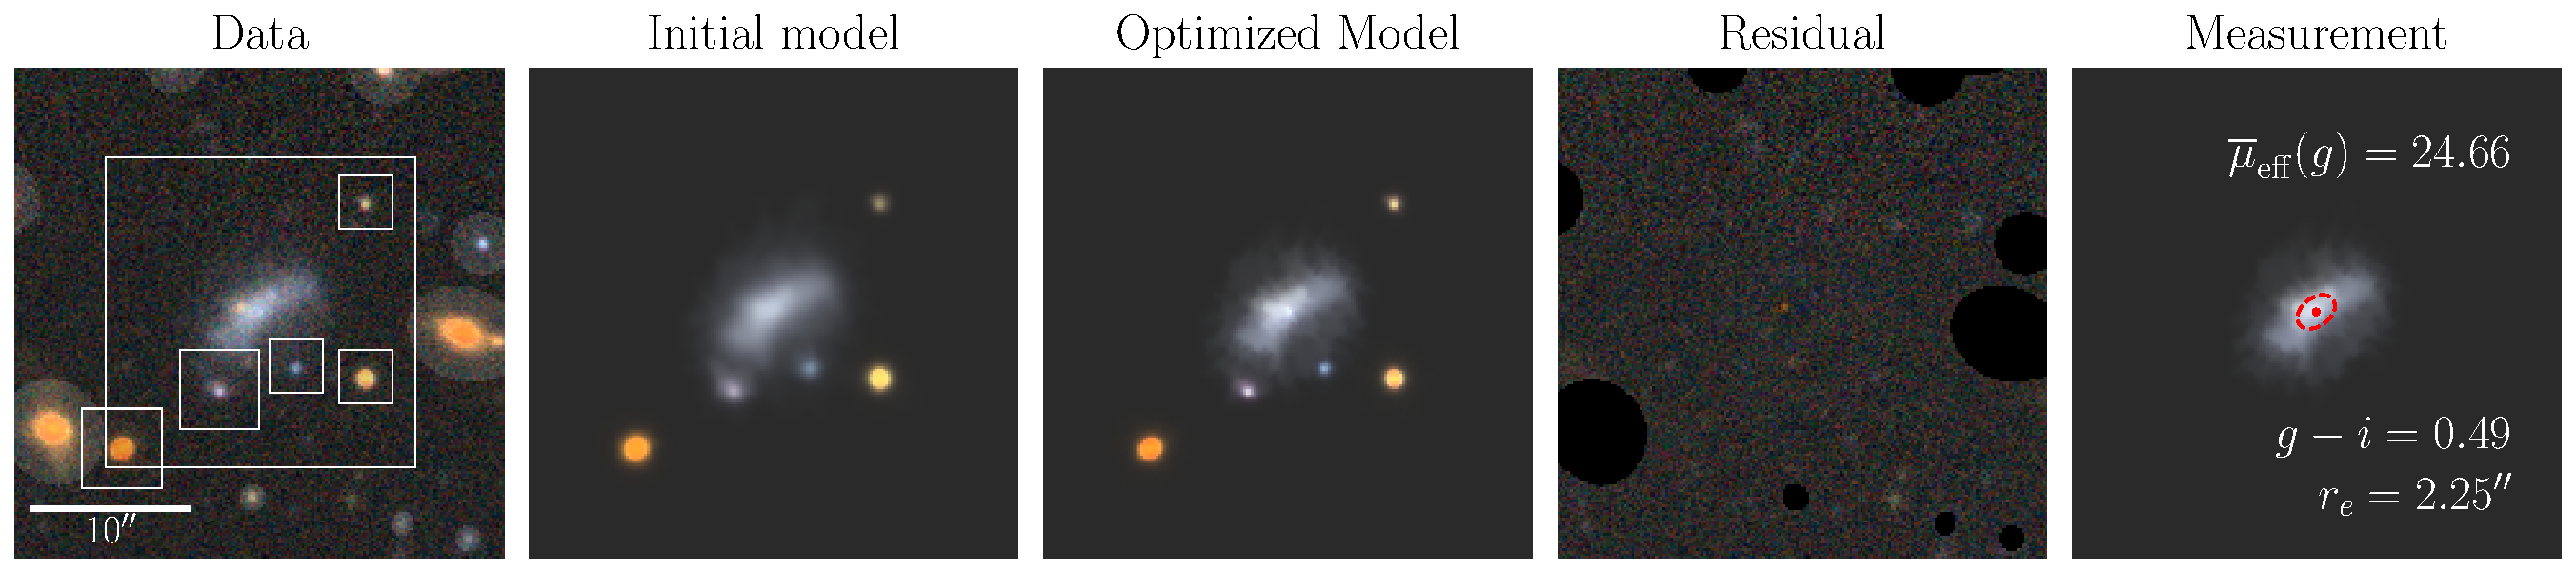
\includegraphics[width=1\linewidth]{vanilla_scarlet_demo.pdf}
		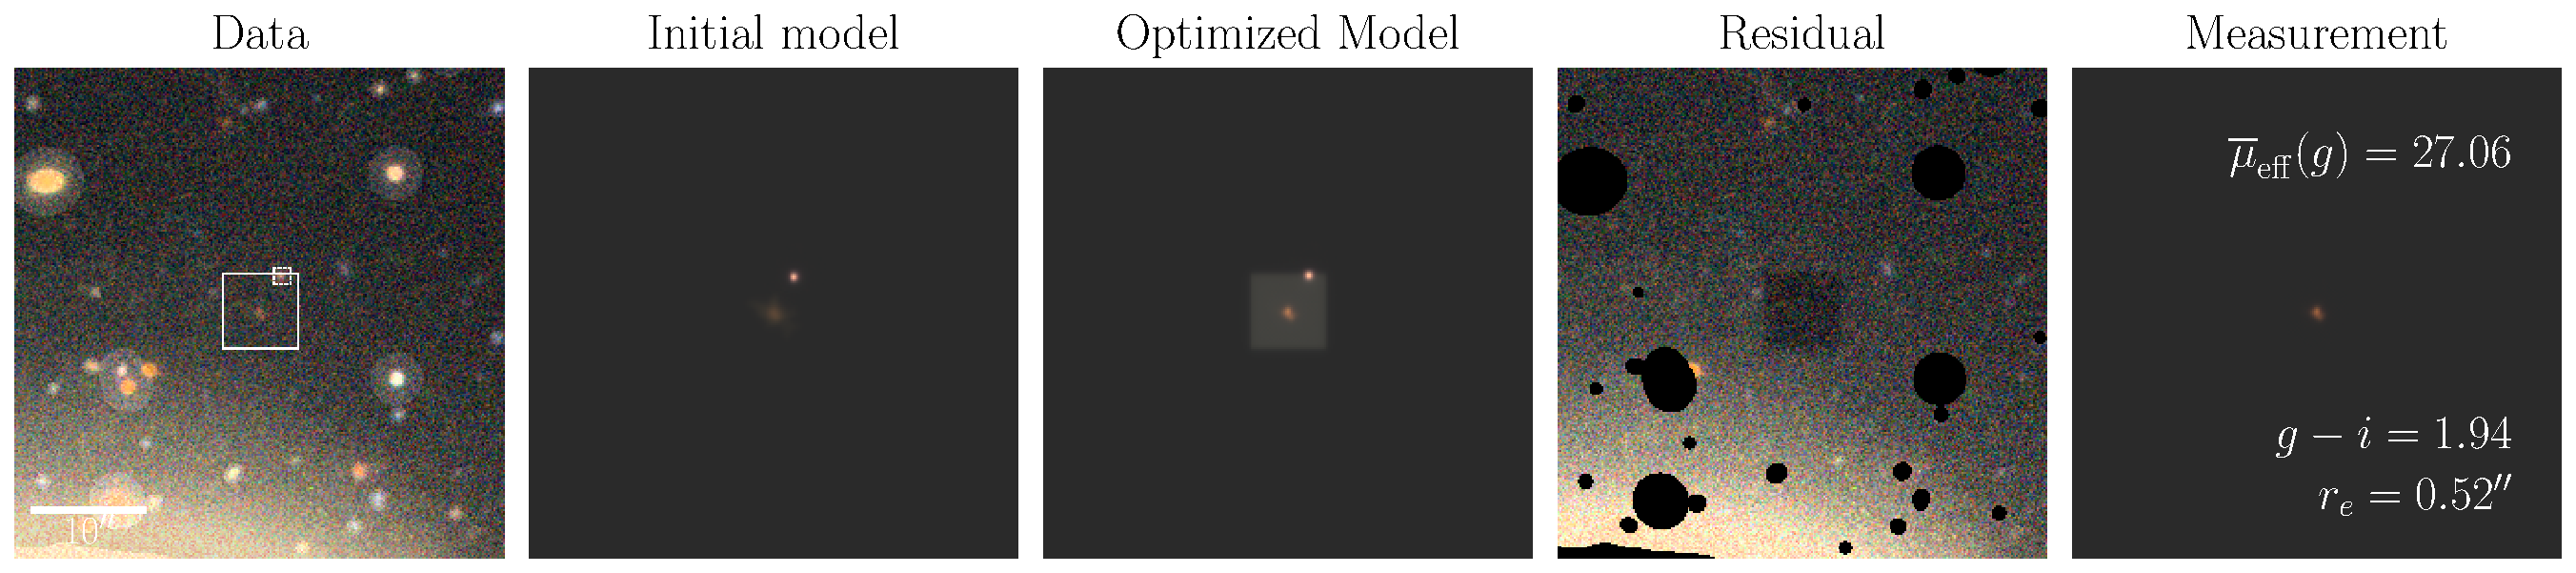
\includegraphics[width=1\linewidth]{vanilla_scarlet_demo2.pdf}
	}
	\caption{A demonstration of the deblending step as described in Section \ref{sec:deblending}. Here we show two objects from our initial sample (Sec \ref{sec:detection}): the one shown in the top panels is a blue LSBG, whereas the one shown in the bottom is a false positive detection which is a blend between high-$z$ galaxy and galaxy outskirts. The data shown in the first column is $griz$ color-composite image with the bounding boxes overlay. The objects covered by the gray shades are masked. The bounding boxes and the initial models (second column) are determined from the smoothed image. The optimized models (PSF convolved) are shown in the third column, the fourth column shows the residual image, and the last column isolates the model of the target object and labels the measured color, size, and surface brightness. After such a deblending step, false positives such as the one in bottom panels can be easily removed based on their measured properties. 
	}
	\label{fig:vanilla_scarlet_demo}
\end{figure*}

After peak detection, there are two more things to be determined before optimization. We need to know which peaks should be modeled, and we would like to initialize the model as best as we can. We note that \code{scarlet} optimizes the model instead of deriving the full posteriors, thus good initialization becomes really important. We tackle these problem as follows. 

The deblending step is designed to model the sources in the vicinity of the target object. Therefore, how large and extended is the target object determines which peaks are relevant. We draw a square bounding box around the target object and include all the peaks inside this box to be modeled. The size of the bounding box is determined as we initialize the model for target object.

We use a multi-extended source with two components to model the target object, such that the model is capable to capture the galaxy structure and color gradient. The source is initialized as follows. We convolve the detection image with a circular Gaussian kernel with $\sigma=1.5$ pixels to boost the contrast between the signal and the sky noise. After smoothing, the LSB outskirts of the target galaxy become more prominent, which helps in determining the bounding box and initializing the morphology matrix. We take the smoothed image and threshold it with $0.1\sigma$ to remove the sky noise. The initial morphology matrix $S_i$ is determined by constructing a symmetric and monotonic approximation to the smoothed image around the target object. The initial SED vector $A_i$ is set to be the sum of the morphology matrices $S_i$ in each band. As a byproduct of initialization, we get a bounding box from $S_i$ which indicates the extent of the target object. Consequently, the size of the bounding box depends on the smoothing kernel and the threshold. We choose the above values by trial and error such that the box is not too large to include many irrelevant peaks, but not too small to lose the flux from the target galaxy. 

Then we take all peaks within the bounding box of the target galaxy and initialize them in the same way. Recall that we have two rounds of peak detection (Sec \ref{sec:peak}), focusing on extended and compact sources respectively. The extended objects detected in the first peak detection step are modeled as single-extended sources. For compact objects that are only detected in the second peak detection, we model them as point sources if their FWHM $<$ 5 pixels, otherwise as compact-extended sources. We also add a flat-sky source to model the local sky around the target. This is helpful for situations where an object overlaps with the LSB outskirts of a bright galaxy (e.g., the bottom panel in Figure \ref{fig:vanilla_scarlet_demo}).

As mentioned above, we only model peaks within the bounding box of the target. However, scattered light from nearby bright stars and galaxies could bias the modeling of sources within the bounding box (e.g., the yellow star in the top left panel of Figure \ref{fig:vanilla_scarlet_demo}). We match our field with the Gaia catalog and mask out stars outside of the bounding box. Since we have already detected peaks throughout the whole cutout image, we also generate a mask for objects outside the bounding box to reduce the impact of scattered light from bright galaxies. 

We demonstrate the above procedures in Figure \ref{fig:vanilla_scarlet_demo} with two examples. The one shown in the top panels is a blue LSBG, whereas the one shown on the bottom is a high-$z$ galaxy blended with the outskirts of a nearby galaxy which falls in our initial sample as a false positive. The first column shows the $griz$ color-composite image \citep{Lupton2004}, where the white boxes mark the bounding box of each source in the scene. The gray shades over objects outside of the target bounding box indicate they are masked out. The second column shows the initial \code{scarlet} models. They look fuzzy because they are constructed from the smoothed image, but they capture the color and the faint outskirts of the LSBG quite well. 

The optimization process uses the adaptive proximal gradient method \citep{Melchior2019}, which is a robust method for optimization with constraints. The model is considered to be converged when the relative changes of parameters are smaller than \code{e\_rel\,=\,2e-4}. Typically, convergence is achieved after $\sim 50$ steps of optimization and the whole modeling takes about 40s for a typical LSBG. It takes longer when the target galaxy has large angular size since more peaks are modeled. The optimized model is shown in the middle column of Figure \ref{fig:vanilla_scarlet_demo} after convolving with the PSF, and the fourth column shows the residual image. The fifth column shows the optimized model only for the target object. 

We notice that the optimized model of the blue LSBG captures its color and morphology quite well. For the false-positive case, the optimized model has a notable bright background thanks to the flat-sky component, and the model for the target itself is very red and compact. The reason why it passes our initial selection is that the galaxy outskirts are shredded by Source Extractor and happen to have a large size and the right color. But once modeled using \code{scarlet}, it becomes clear that this is just a false positive detection and should be removed. 

% As a result of such initialization, we only optimize the object function $f$ defined for sources within the bounding box of the target object. 
% \textbf{For bright sources? Cookie cutter effect? I don't think cookie cutter is important here.}

\subsubsection{Measurement and false positive removal}\label{sec:non-par-measurement}

\begin{figure*}
	\vbox{
		\centering
		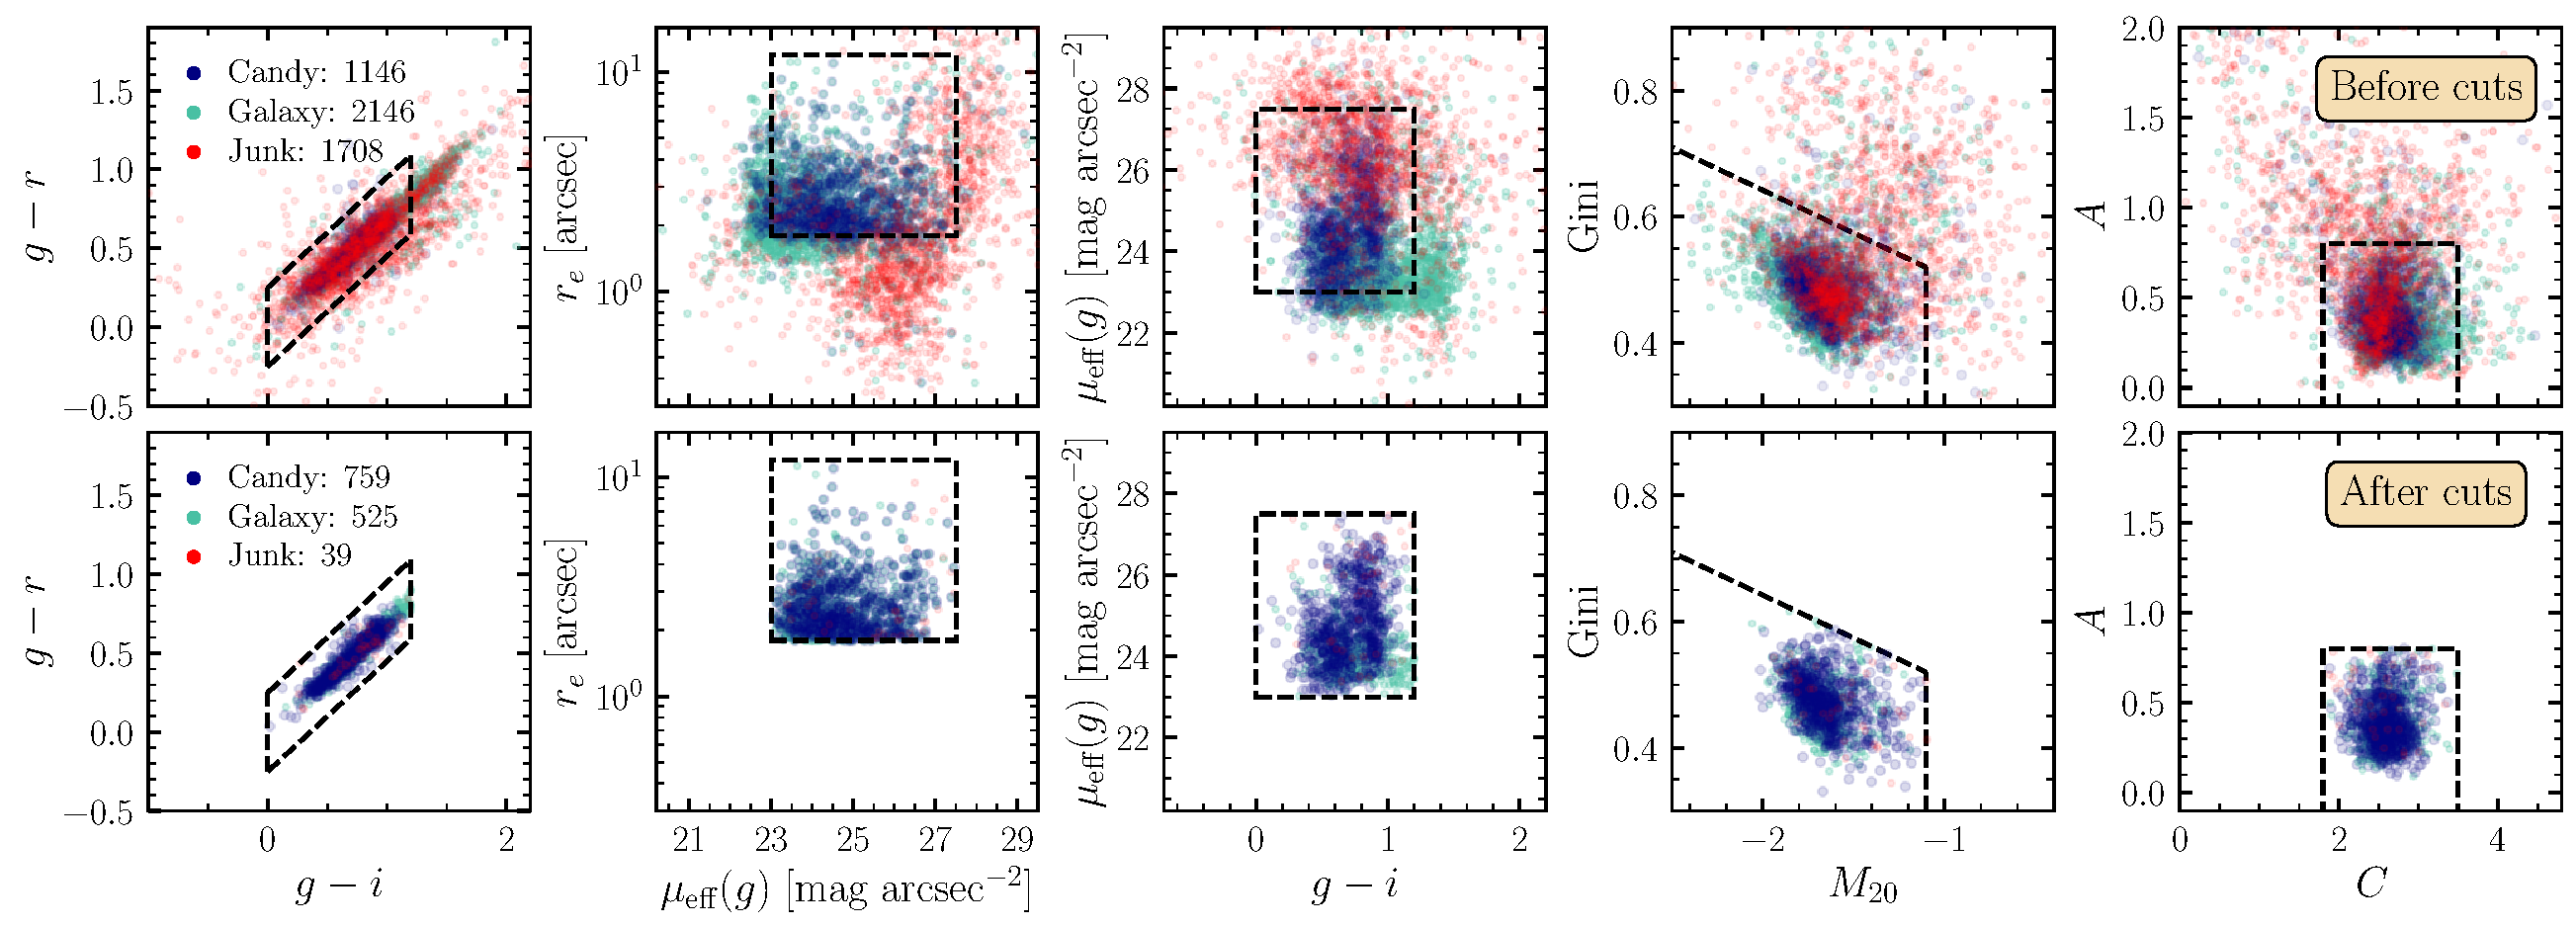
\includegraphics[width=1.0\linewidth]{deblending_cuts.pdf}
	}
	\caption{The distribution of LSBG candidates from our initial sample in the parameter space as measured from the \code{scarlet} models. We visually inspected 5,000 LSBG candidates and labeled them as \code{candy} (LSBGs with typically dwarf galaxy features), \code{galaxy} (higher surface brightness galaxies or galaxies with spiral galaxy features), and \code{junk} (false positives). We propose a selection based on size, color, surface brightness and morphology (dashed boxes) to effectively remove false positives but still achieves a high completeness. After such cuts (bottom panels), 97\% of false positives and 75\% of non-LSB galaxies are removed according to our visual inspection results. 
	}
	\label{fig:deblending_cuts}
\end{figure*}

After running the vanilla scarlet for LSGB candidates, we successfully deblend the target object from nearby sources. Unlike other modeling codes, the non-parametric \code{scarlet} model is very flexible on modeling galaxies with complex structures. But the non-parametric nature means that we have to make our own measurements to quantify the size and shape of the \code{scarlet} model. As shown in the last column of Figure \ref{fig:vanilla_scarlet_demo}, we take out the model of the target object and analyze it using \href{https://statmorph.readthedocs.io/en/latest/}{\code{statmorph}} \citep{statmorph}. The purpose of this analysis is to extract the structural and morphological parameters of the target object. We further use these diagnostics to remove false positives. 

\code{Statmorph} calculates non-parametric morphological and structural parameters, including effective radius, concentration-asymmetry-smoothness statistics \citep[CAS,][]{Conselice2003}, and Gini-M20 \citep{Abraham2003,Lotz2004}. The measurement requires an image, a variance map, and a PSF. For our purpose, the ``image'' is just the \code{scarlet} model convolved with the observed PSF. The variance map and PSF are taken from HSC cutouts. We also force the sky level to be zero because sky has already been fit when running vanilla scarlet. 

One of the most important diagnostics is the effective radius of the object. In this paper, we refer to effective radius as the circularized effective radius $r_{e}$, defined as the $r_{e} = r_{\rm eff, sma} \sqrt{b/a}$ where $r_{\rm eff, sma}$ is the effective radius measured along the semi-major axis of the aligned elliptical isophotes, and $b/a$ is the axis ratio of the isophotes. In \code{statmorph}, the effective radius is calculated using elliptical apertures, where the ellipticity $\varepsilon$ is determined by calculating the second moment of the image. The total magnitudes are simply calculated by summing up the model in each band, and colors are defined using total magnitudes.\footnote{Galactic extinction correction is not applied at this point.} The central surface brightness $\mu_0$ is measured by extrapolating the surface brightness profile to $r\to 0$. We define the average surface brightness within the effective radius as $\mu_{\rm eff} = m - 2.5 \log_{10}(2 \pi r_e^2)$, where $m$ is the total magnitude. 

We also use the Gini-M20 and CAS statistics. The Gini coefficient and M20 statistics \citep{Abraham2003,Lotz2004} quantify how concentrated/extended the flux distribution is across the image. The CAS statistics characterize the concentration $C$, asymmetry $A$, and smoothness $S$ of the light distribution of the object. We refer the readers to \citet{statmorph} for more details on their definitions and implementations. The morphological and structural parameters are the same in different bands by construction in the \code{scarlet} model.

To better guide us on how to use these diagnostics, we visually inspect a subset of LSBG candidates in our initial sample (Sec \ref{sec:detection}) and use the labels to construct the metrics. We randomly selected 5,000 LSBG candidates that are matched with a MW-like host at $0.01 < z < 0.04$ in NSA catalog (see Sec \ref{sec:match} for details). We run vanilla scarlet for all of them and measure morphological parameters as described above. Then we do visual inspection by looking at the $griz$ color-composite images with 0.5 arcmin on a side. Objects are classified into three types: \code{candy} (LSB galaxies with typically dwarf galaxy features), \code{galaxy} (high surface brightness galaxies, or galaxies with spiral galaxy features), and \code{junk} (false positives, including tidal streams, galaxy outskirts blends, and other artifacts). The difference between \code{candy} and \code{galaxy} can be quite ambiguous. 

The visual inspection was done by coauthors JEG, JG, SH, RB, KC, AG, and EKF. Each object has been inspected by at least one person. In the end, we combine the votes from different people. An object is classified as \code{junk} if the number of votes as \code{junk} is larger than the number of votes as \code{candy} and \code{galaxy}. For objects that are not \code{junk}, if the number of votes as \code{candy} is greater than the votes as \code{galaxy}, we classify this object as \code{candy}. Everything else is classified as \code{galaxy}. In total, there are 1146 \code{candies}, 2146 \code{galaxies}, and 1708 \code{junk}. 

We use these visual inspection results to teach us how to use the morphological and structural diagnostics. The distributions of \code{candy} (blue), \code{galaxy} (green), and \code{junk} (red) in the parameter space are shown in the top panels of Figure \ref{fig:deblending_cuts}. Although \code{junk} is scattered throughout the parameter space, a large fraction of the junk comprises small things with very red colors, very faint surface brightness, large concentration and large asymmetry. Therefore, we come up with the following selection cuts to remove the false positives:
\begin{itemize}
    \item Color:
    \[0.0 < g-i < 1.2,\quad |(g-r) - 0.7\cdot (g-i)| < 0.25\]
    \item Size: \[1.8 \arcsec < r_e < 12 \arcsec\]
    \item Surface brightness: \[\mu_0(g) > 22.5,\quad 23.0 < \mu_{\rm eff}(g) < 27.5,\]
    \item Morphology: 
    \begin{gather*}
        \varepsilon < 0.65,\quad \mathrm{Gini} < 0.70,\quad M_{20} < -1.1,\\
        \mathrm{Gini} < -0.136\cdot M_{20} + 0.37,\\
        1.8 < C < 3.5,\quad A < 0.8.
    \end{gather*}
\end{itemize}
These criteria (shown as dashed lines in Figure \ref{fig:deblending_cuts}) effectively help us remove objects that are not likely to be LSBGs of interest. The color cuts here are narrower than the one used in the initial detection (Sec \ref{sec:detection}) to further remove junk and background high redshift galaxies. We not only remove objects with small sizes, but also exclude objects with large size, very low surface brightness, and high concentration. This is because the scarlet models of some junk can be very concentrated in the center but also very extended. The slant demarcation line on the Gini-$M_{20}$ diagram is motivated by the line used in \citet{Lotz2008} to separate merging galaxies from normal galaxies. 

The bottom panels in Figure \ref{fig:deblending_cuts} show the objects after applying the above selections. With these cuts, 97\% of the false positives are removed, but the majority (70\%) of \code{candy} still remains. The number of \code{galaxy} also drops by 75\%. This empirical selection based on the non-parametric measurements on the scarlet models successfully removes most of the false positives and a large fraction of background galaxies in our initial sample. Furthermore, the completeness of real LSBG detection remains high. In Section \ref{sec:completeness}, we characterize the completeness of this ``deblending'' step by injecting mock \sersic{} galaxies, and we achieve $\sim80\%$ completeness at $\sbeff = 27.0\ \sbunit$ and $>50\%$ completeness at $\sbeff = 27.5\ \sbunit$ (Fig. \ref{fig:completeness}). We emphasize that the vanilla scarlet modeling and non-parametric measurements are not designed to recover the intrinsic properties of the galaxies. They are used only as a diagnostic tool to remove false positives. We perform more detailed modeling in Section \ref{sec:modeling} to measure galaxy properties for science. 


We notice that many other works have been using machine learning (ML) algorithms to classify LSBG candidates and exclude spurious detection. Among others, \citet{Tanoglidis2021} take the output catalog from \code{Source Extractor} and use the Support Vector Machine algorithm to classify objects in their initial sample and reduce the number of objects that are visually inspected. \citet{Zaritsky2019,Zaritsky2021,Zaritsky2022} use convolutional neural networks to classify LSBGs into binary classes based on their images. These endeavors certainly help reducing the human labor on visually inspecting tens of thousands of objects. However, training such a supervised ML algorithm relies on the labeled data which should also sample the parameter space evenly. Once labels are assigned (e.g., LSBG v.s. non-LSBG), there will be little way to change later. On the contrary, our cuts based on the measured properties can be tweaked to be more complete (including more junks) or be more pure (aggressive cuts) depends on the specific science goal. The visual inspections only guide us to design those metrics. This measurement-based method is more intuitive, reproducible, and transferable. We will also explore machine learning methods and compare with our deblending cuts in future works. We would also like to utilize the information about the Milky Way dust to exclude spurious detection on Galactic cirrus \citep{Zaritsky2021,Zaritsky2022}.

% Tanoglidis doesn't estimate measurement uncertainty. Doesn't systematically estimate completeness, only validates the comp using deeper fornax observations. Also, the artifact of HSC is less compared with DES/DECaLS?
% SMUDGES: Their sample might be cleaner thanks to their wavelet detection emphasizing specific spatial frequency. But they still need a lot of visual inspection.

\subsection{Modeling}\label{sec:modeling}
Although the vanilla scarlet modeling provides useful information to help us remove false positives, it does not necessarily give us unbiased estimations on size, color, total magnitude, etc. In fact, the vanilla scarlet model usually under-estimates the size and the total flux of LSB objects. This is because the faint outskirts of LSBGs are typically not modeled well due to the non-parametric nature of vanilla scarlet. We elaborate this point as follows.

When doing parametric modeling such as \sersic{} fitting, we effectively apply radial averaging within elliptical annulus and boost the SNR by binning pixels. In other words, pixels within the same isophotal annulus are assumed to have the same intensity thus are strongly correlated. However, the non-parametric nature of vanilla \code{scarlet} only assumes monotonicity, which imposes quite weak correlations among pixels. Consequently, it is very hard for the non-parametric modeling to probe down to very low surface brightness features. Furthermore, the monotonicity constraint stops the model from growing in certain directions if there is another source along this direction, otherwise monotonicity is broken. This issue, dubbed the ``cookie-cutter effect'', can be seen in the third column of Figure \ref{fig:vanilla_scarlet_demo} where the model of the target object never exceeds the other objects next to it. As a result, the non-parametric model often does not capture the LSB outskirts of LSBG, thus biasing the measurements. In the following, we explore a novel method to perform parametric fitting while exploiting the advantages of \code{scarlet}.

A traditional way of doing parametric modeling is to first mask out contaminants based on the detection segmentation map, then fit a model to the masked image. However, the fitting results are very sensitive to the masking scheme \citep[e.g.,][]{Greco2018} and sky background. A possible solution to this problem is to simultaneously model all the objects in the cutout and the sky using parametric models (e.g., in DECaLS, \citealt{Dey2019}). In this work, we combine the advantage of parametric modeling with the power of deblending in \code{scarlet}. To be specific, we follow the spirit of deblending as described in Section \ref{sec:deblending}, but replace the non-parametric model for the target with a parametric model. In this way, the LSB outskirts of LSBGs can be better captured with the parametric model and the impact of contaminants is minimized because they are modeled simultaneously. The parametric model for the target object does not suffer from the ``cookie-cutter'' issue any more. 

We use the Spergel surface brightness profile \citep{Spergel2010} to model the LSBGs. The Spergel profile is motivated by having a simple analytical expression in the Fourier space, making it easy to be convolved with a PSF\footnote{On the opposite, the \sersic{} profile does not have a simple analytic form in the Fourier space.}. The surface brightness of a Spergel profile has a form of
\begin{equation}
    \label{eq:spergel}
    I_\nu(r) = \frac{c_{\nu}^{2} L_{0}}{2\pi r_{0}^{2}} f_{\nu}\left(\frac{c_{\nu} r}{r_{0}}\right),
\end{equation}
where 
\begin{equation}
    f_{\nu}(u)=\left(\frac{u}{2}\right)^{\nu} \frac{K_{\nu}(u)}{\Gamma(\nu+1)},
\end{equation}
and $K_\nu(u)$ is the Modified Bessel function of the second kind. The half-light radius is $r_0$, the total luminosity is $L_0$, and $c_\nu$ satisfies the equation $(1 + \nu)f_{\nu + 1}(c_\nu) = 1/4$. Similar to the \sersic{} index, the parameter $\nu$ (dubbed as ``Spergel index'') controls the concentration of the light profile. As shown in Appendix \ref{ap:spergel}, the Spergel profile approximates the \sersic{} profile very well over the range of \sersic{} index that is relevant to the study of LSBGs.

We initialize the Spergel model for the target object differently, while other objects are still initialized in the same way as in the deblending step (Section \ref{sec:deblending}). First, we initialize a vanilla scarlet model for the target object, and we measure the effective radius $r_e$, total flux, and the shape of the scarlet model. We use these numbers to initialize the Spergel profile. The size of the bounding box is also updated to be the maximum between 250 pixels and $10\, r_e$. Peaks within this bounding box (other than the target) are modeled using vanilla scarlet. For the target, we still require positivity constraint, and the monotonicity is automatically satisfied by the Spergel profile. 

After optimization, we take the $r_0$ in Equation \eqref{eq:spergel} as the circularized half-light radius $r_e$, and take $L_0$ as the total flux. The average surface brightness $\overline{\mu}_{\rm eff}$ is calculated in the same way as in Section \ref{sec:non-par-measurement}. In the following section, we assess the quality of the Spergel modeling by injecting mock \sersic{} galaxies and comparing the recovered properties with truth. 

\textbf{
Based on the modeling results, we apply the same color cuts as in Section \ref{sec:deblending} and a size cut of $1.6\arcsec < r_e < 15\arcsec$ to further remove unreliable fits and false positives. }
\jiaxuan{Check if this is considered in the completeness.}

\subsection{Completeness and Measurement Uncertainty}\label{sec:comp_meas}
The completeness of the LSBG search is important not only for understanding our searching efficiency and improving the method in the future but also for deriving the completeness-corrected results for LSBG sciences. Similar to many other works \citep[e.g.,][]{Zaritsky2021,CarlstenELVES2022,Greene2022}, we derive the completeness by simulating mock LSBGs and try to recover them from the image. Using these mock galaxies, we also characterize the measurement bias and uncertainty by comparing the measured properties with the truth. 


\subsubsection{Completeness}\label{sec:completeness}
\begin{figure*}
	\vbox{ 
		%\vskip -10mm
		\centering
		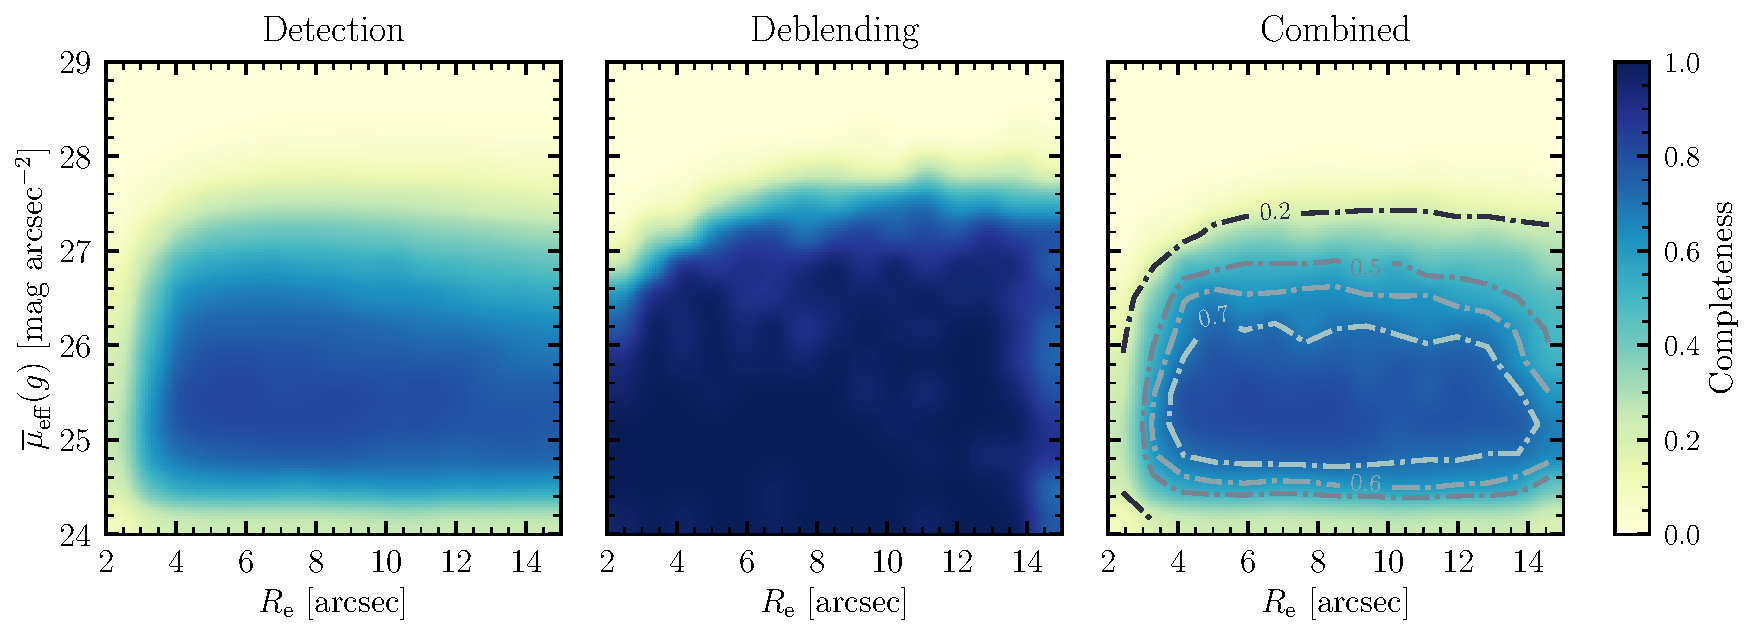
\includegraphics[width=1\linewidth]{completeness.pdf}
	}
	\caption{The completeness of our LSBG search as a function of effective radius $r_e$ and the average surface brightness $\sbeff$. We characterize the completeness by injecting mock \sersic{} galaxies into coadd images. The overall completeness (right panel) comprises the detection completeness (left panel, see Sec. \ref{sec:detection}) and deblending completeness (middle panel, see Sec. \ref{sec:deblending}) where false positives are removed. The dashed lines in the right panel highlight the 70\%, 50\%, and 20\% completeness contours. The completeness drops for smaller sizes and faint surface brightness. We are $>70\%$ complete to $\sbeff < 26.5\ \sbunit$ and $3\arcsec < r_e < 14\arcsec$, and $>50\%$ complete to $\sbeff \leqslant 27.0\ \sbunit$. The completeness drops as we go to fainter surface brightness and smaller size. 
	%The mock galaxies span a large range in size, surface brightness, \sersic{} index, color, and ellipticity. 
	}
	\label{fig:completeness}
\end{figure*}

A real LSBG can be missed in the detection step (Sec. \ref{sec:detection}) or be excluded in the deblending step (Sec. \ref{sec:deblending}). Thus, the overall completeness is a combination of detection completeness and deblending completeness. We performed a large suite of image simulation to derive the completeness. The detection completeness is defined as the number of detected objects divided by the number of injected objects, whereas the deblending completeness is defined as the fraction of objects remaining after the deblending cuts. 

For the detection completeness, we inject $\sim 700,000$ mock galaxies with single \sersic{} light profiles \citep{Sersic1963} into the coadd images\footnote{We have also done extensive tests on injecting mock galaxies into the raw images and going through the entire data reduction pipeline. This is very expensive in terms of both CPU time and disk space, since we must run the full \code{hscPipe}. However, we find no noticeable difference in the completeness between this method and the direct injection to coadd images.}. The mock galaxies follow uniform distributions in size ($2\arcsec \leqslant r_{e} \leqslant 21\arcsec$), surface brightness ($23 \leqslant \overline{\mu}_{\rm eff}(g) \leqslant 28.5\ \mathrm{mag\ arcsec^{-2}}$), \sersic{} index ($0.8 < n < 1.2$), and ellipticity ($0 < \varepsilon < 0.6$) by resembling the LSBG distribution in \citetalias{Greco2018}. They are randomly assigned to have a blue ($g-i=0.47,\ g-r=0.32$), medium ($g-i=0.64,\ g-r=0.43$), and red ($g-i=0.82,\ g-r=0.56$) color with equal chance. Then we run the detection step as described in Sec. \ref{sec:detection} and cross-match the detection catalog with the input mock galaxy catalog to calculate completeness. We split the size and surface brightness range into 15 bins with $\Delta r_e = 0.86\arcsec$, $\Delta \sbeff = 0.33\ \sbunit$, and interpolate over bins using an isotropic Gaussian kernel with $\sigma = 0.5$. We notice that the size and surface brightness shown in Figure \ref{fig:completeness} are all the intrinsic values for the mock galaxies, which are different from the measured ones. We discuss measurement biases in Section \ref{sec:meas_unc}.

We find that the detection completeness mainly depends on the size and surface brightness. As shown in the left panel of Figure \ref{fig:completeness}, the detection completeness remains high across different sizes. It drops below 50\% when the surface brightness gets fainter than $\sbeff = 27.5\ \sbunit$. We find negligible dependence of completeness on \sersic{} index, color, and ellipticity. Therefore, we neglect the dependence of detection completeness on parameters other than size and surface brightness hereafter.\footnote{We performed a smaller set of image simulation where we extend the ellipticity range and also simulated galaxies with additional structures (such as star-forming clumps). We find the completeness declines for $\varepsilon > 0.6$, suggesting that edge-on disk galaxies may be missing from our sample. Please see \citet{Greene2022} for more details.}

For the deblending completeness, we inject 5,000 mock \sersic{} galaxies into the coadd and run vanilla scarlet on them. The mock galaxies follow the same uniform distribution in size, surface brightness, ellipticity, \sersic{} index as for deriving the detection completeness, but follow a Gaussian distribution in color: $g-i \sim \mathcal{N}(0.6, 0.2^2),\ g-r = 0.7 (g-i) + \mathcal{N}(0, 0.03^2)$. We measure the size and surface brightness on the scarlet models of the mock galaxies, then we apply the deblending cuts. The deblending completeness as a function of size and surface brightness is shown in the middle panel of Figure \ref{fig:completeness}. The deblending completeness is very high at the bright end, but starts to decline with increasing size and surface brightness. Mock galaxies fainter than $\sbeff > 27.5\ \sbunit$ are mostly removed by the deblending step, likely due to the blending of other small compact sources with the mock galaxy. Interestingly, the detection completeness and deblending completeness all drop below 40\% around $\sbeff=27.5\ \sbunit$. In this sense, the detection and deblending cooperate well in terms of completeness. 

The combined completeness is shown in the right panel of Figure \ref{fig:completeness}. The dashed lines highlight the 70\%, 50\%, and 20\% completeness contours. The completeness drops as we go to fainter surface brightness and smaller size. We are $>70\%$ complete to $\sbeff < 26.5\ \sbunit$ and $3\arcsec < r_e < 14\arcsec$, and $>50\%$ complete to $\sbeff \leqslant 27.0\ \sbunit$. Although \sersic{} galaxies do not necessarily resemble the morphology of real LSBGs, our completeness based on \sersic{} model still sets a baseline or upper limit on the real completeness. In the future, we might be more capable of generating realistic LSBGs using deep learning techniques (e.g., diffusion model). 


We compare our completeness with that of other LSBG searches. Our completeness is most similar to \citetalias{Greco2018}, where they also reach $\sim 50\%$ at $\sbeff \approx 27.0\ \sbunit$ and $3\arcsec < r_e < 12\arcsec$ \citep{Kado-Fong2021,Greene2022}, but their completeness decreases more as increasing size. \citet{CarlstenELVES2022} use a similar searching algorithm to \citetalias{Greco2018} and ours and reach a completeness of $\sim 50\%$ at $\mu_0(g)\approx 26.5\ \sbunit$ or equivalently $\sbeff = 27.5\ \sbunit$. \citet{vdBurg2017} searched LSBGs from the ESO Kilo-Degree Survey data and achieved $\sim 50\%$ completeness at $\sbeffr\approx 26.0\ \sbunit$ or equivalently $\sbeff \approx 26.6\ \sbunit$. \citet{Zaritsky2021} focus on searching LSBGs in SDSS Stripe82 region using the Dark Energy Camera Legacy Survey (DECaLS, \citealt{Dey2019}) survey and reach $\sim 25\%$ completeness at $\mu_{0}(g) \approx 25.5\ \sbunit$ or equivalently $\sbeff \approx 26.5\ \sbunit$. Their low completeness might be explained by the fact that they remove a large fraction of the sky covered by the Galactic dust. \citet{Tanoglidis2021} conducted LSBG search using the Dark Energy Survey (DES, \citealt{Abbot2018}) data and conclude an overall completeness of $\sim 40\%$ by comparing their catalog with the deeper observations in the Fornax cluster. \citet{Kado-Fong2021} estimate the completeness of \citet{Tanoglidis2021} by comparing with \citetalias{Greco2018} and find a completeness similar to \citetalias{Greco2018} at $\sbeff = 25.5\ \sbunit$ but much smaller completeness above $\sbeff > 26.5\ \sbunit$. In summary, our search achieves an overall high completeness compared with other works, and we demonstrate the great potential of HSC data on LSBG studies. 
\jiaxuan{also cite dragonfly}

\subsubsection{Measurement bias and uncertainty}\label{sec:meas_unc}


% \begin{figure*}
% 	\vbox{ 
% 		\centering
% 		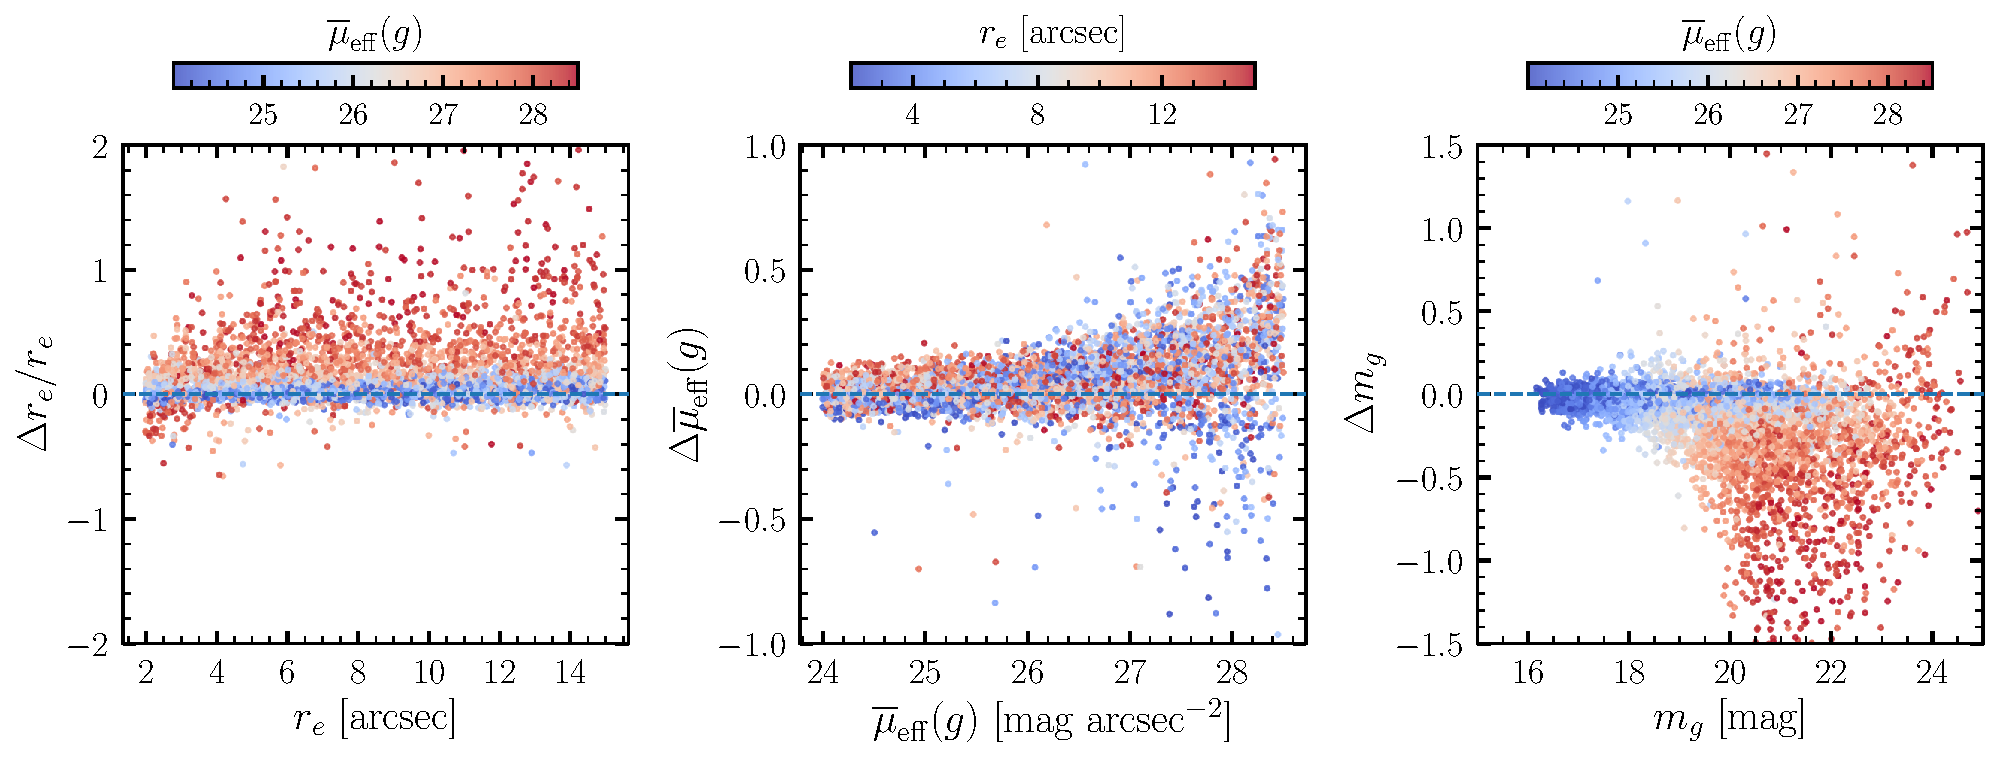
\includegraphics[width=1\linewidth]{meas_bias.pdf}
% 	}
%     \caption{Caption}
%     \label{fig:meas_bias}
% \end{figure*}

\begin{figure*}
	\vbox{ 
		\centering
		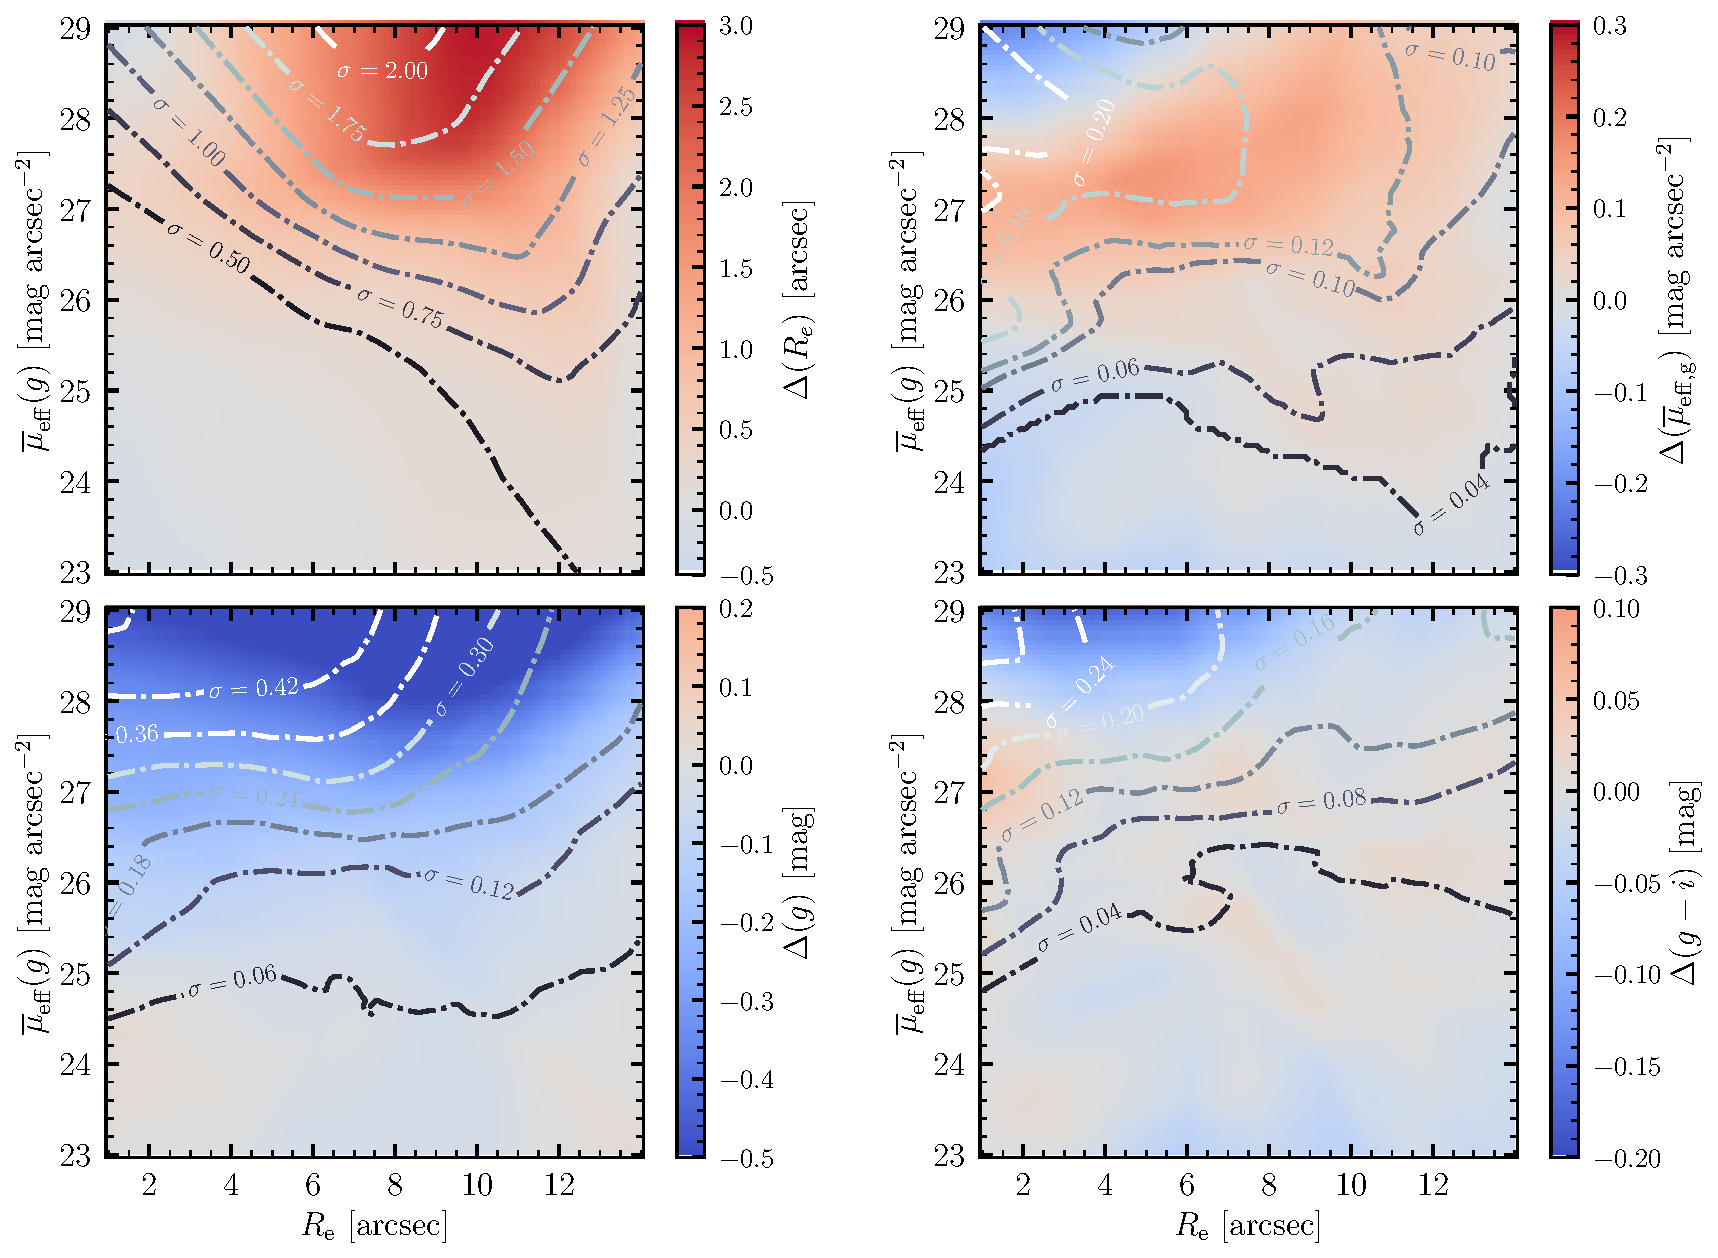
\includegraphics[width=1\linewidth]{meas_error_spergel.pdf}
	}
    \caption{The measurement bias and uncertainty as a function of measured angular size $r_e$ and surface brightness $\sbeff$. The colors show the bias term while the dashed contours show the constant uncertainty lines. We derive the bias of total magnitudes from the biases of $r_e$, $\sbeff$, and colors consistently. We find that the bias and uncertainty of our measurement increase toward the fainter end. We apply the bias correction to the real LSBGs before studying their physical properties.}
    \label{fig:meas_err}
\end{figure*}


Due to the low surface brightness nature of LSBGs, their size, magnitude, surface brightness and shape are hard to characterize and are typically associated with large uncertainties. \citet{Haussler2007} use mock single-\sersic{} galaxies and parametric fitting codes to demonstrate that the estimated size and total magnitude are sensitive to local sky estimation and masking of neighboring objects. In the low surface brightness regime, the measured size and total magnitude can be quite biased and have large uncertainties. Therefore, measurement bias and uncertainty must be considered when studying the properties of LSBGs. \citet{Zaritsky2021,Zaritsky2022} characterize their measurement bias and uncertainty by injecting mock \sersic{} galaxies into the coadd and compare the recovered properties with the truth. \citet{Tanoglidis2022ICML} recently propose a new method to estimate the measurement error using a Bayesian Neural Network. In this paper, we simply take the former method because of its simplicity. 

In order to test how well we recover the photometric and structural parameters in the our measurement (Sec \ref{sec:modeling}), we take the 5,000 mock \sersic{} galaxies used for computing the deblending completeness and model them using the Spergel light profile. We compare the fitting results with the ground truth, and we find that the measured effective radius $r_e$ is biased to be smaller than the truth, and the bias depends on the surface brightness and the angular size. For surface brightness fainter than $27\ \sbunit$, the measured size can be much smaller than the truth. As a result, the total magnitude $m$ and the average surface brightness $\overline{\mu}_{\rm eff}$ are also measured to be fainter than the truths. 

Similar to \citet{Zaritsky2021}, we model the bias and uncertainty in size, surface brightness, total magnitude, and color as a function of other parameters including size, surface brightness, and shapes. However, we do not find any significant dependence of the bias on color, ellipticity, and Spergel index. Thus we just model the bias and uncertainty as a function of the \textit{measured} angular size $r_e$ and surface brightness $\sbeff$.

Given the size and surface brightness of our simulated galaxies, we set the ranges of the observed size and surface brightness to be $r_e\in[1\arcsec, 15\arcsec],\ \sbeff\in[23, 29]$. We then split the observed $r_e-\overline{\mu}_{\rm eff}(g)$ plane using an $8\times 8$ grid, and calculate the mean bias $\Delta X = X_{\rm truth} - X_{\rm meas}$ within each bin, where $X=\{\sbeff,\ g-i,\ g-r\}$. For $r_e$, we calculate the relative bias $\Delta r_e / r_e$ instead because it is less dependent on the angular size. Then we interpolate over the grid using a multi-quadratic kernel\footnote{\url{https://docs.scipy.org/doc/scipy/reference/generated/scipy.interpolate.RBFInterpolator.html}}. Unlike \citet{Zaritsky2021} where they fit models in 4-D space, we find interpolation working well enough in the 2-D space and do not use polynomial fitting to avoid meaningless results outside of the fitting range. We emphasize that the bias and uncertainty are modeled to be functions of the measured properties, not intrinsic ones, such that we can correct for bias based on our measurements. 

In Figure \ref{fig:meas_err}, the colors show the interpolated bias terms as a function of the measured size and surface brightness. The size and surface brightness bias grows with increasing surface brightness. The bias term is not a monotonic function of size because the size here is not intrinsic size. It is the bias in size measurement that makes galaxies with large intrinsic $r_e$ pile up around $r_e\sim 6\arcsec$. We also find the bias in $g-i$ color quite small. 

For LSBGs in our sample, we apply corrections for the bias using the interpolated bias terms. We first correct for the bias in size, $g$-band average surface brightness, $g-r$ and $g-i$ colors. Then we calculate the $g$-band total magnitude following $m_g = \overline{\mu}_{\rm eff}(g) - 2.5\log(2\pi r_e^2)$. The magnitudes and surface brightnesses in other bands are derived using $g$-band magnitude, surface brightness, and colors. In this way, we apply a self-consistent correction for the measurement biases to the data. 

The measurement uncertainty consists of a statistical uncertainty which is determined by the shape of the likelihood (posterior) surface, and a systematic uncertainty which is related to various factors including sky subtraction, neighboring contamination, etc. Unlike other parametric modeling codes, \code{scarlet} does not explore the full posterior space but rather finds one optimal solution. Thus we have no access to the statistical error on the measured properties from \code{scarlet}. Fortunately, by comparing the recovered properties of mock galaxies with the truth, we can empirically estimate the measurement uncertainty without knowing the impact of each factor. Following the same method as that of calculating the bias, in each bin we compute the $1\sigma$ standard deviation of the difference between the truth and the bias-corrected measurement, then we interpolate over the grid. The measurement errors $\sigma(X)$ are shown in Figure \ref{fig:meas_err} as contours, and they have the same units as the biases. We set minimum uncertainties to be $\sigma(r_e) \geqslant 0.3,\ \sigma(\overline{\mu}_{\rm eff}) \geqslant 0.05,\ \sigma(g-i) \geqslant 0.05$ to avoid meaningless uncertainty due to small statistics.

In the following sections, we apply the bias corrections to the real LSBGs, estimate the measurement uncertainties, and evaluate the completeness based on bias-corrected properties. We also incorporate the measurement errors into the science figures. The values presented in our catalogs are already bias-corrected, but we do provide the bias values for reference. 



\jiaxuan{say somewhere in the results section that only SMUDGES measured and corrected measurement bias. vdB 16 doesn't consider whether GALFIT gives the corrrect $R_e$}

\section{UDGs and UPGs in Milky-Way analogs}\label{sec:sample_construction}
The goal of this paper is to study the diffuse galaxies hosted by MW-like galaxies. However, one of the major obstacles for studying LSBGs is that it is hard to get distance information. Beside direct distance measurements (e.g., SAGA, ELVES, \citealt{Kadowaki2021}), it is common to assume a distance to a dwarf candidate by associating it with a host galaxy based on the projected angular distance \citep[e.g.,][]{vanDokkum2015,vdBurg2016,Wang2021,Zaritsky2022,Nashimoto2022}. A statistical background subtraction is then needed to account for the contribution from background and foreground galaxies. Cross-correlation between the LSBG sample and a host galaxy sample can also reveal the distance distribution of LSBGs \citep{Greene2022}. These methods are also complemented by machine learning techniques \citep{Baxter2021,xSAGA-I}. In this Section, we cross-match our LSBG catalog with MW-like galaxies in the NSA catalog and construct the UDG and UPG sample. 

\subsection{Matching with Milky-Way analogs}\label{sec:match}
The properties of the Milky Way itself vary in the literature \citep{Licquia2015,Bland-Hawthorn2016} and the definitions of MW analogs are different among different studies. In the SAGA survey \citep{SAGA-I,SAGA-II}, MW analogs are selected based on their absolute $K$-band magnitude $-23 > M_K > -24.6$, which is derived using abundance matching by assuming a simple galaxy-halo connection model (Fig. 2 in \citealt{SAGA-I}). This luminosity range approximately corresponds to a stellar mass range of $10.2 < \log\, M_\star/M_\odot < 11.0$. They also require the MW analogs to be in isolation (without nearby bright galaxies) and lie in a redshift range of $0.005 < z < 0.01$ (20--40 Mpc). In the ELVES survey \citep{ELVES-I,ELVES-II,CarlstenELVES2022}, the requirements for MW-like host is loosened to be $M_K < -22.1$~mag ($M_\star > 10^{9.9}\ M_\odot$) because the probed volume by ELVES ($D<12$ Mpc) is smaller than that of SAGA. In this work, we choose the stellar mass range of MW analogs to be $10.2 < \log\, M_\star/M_\odot < 11.2$, which is simply a 1 dex bin centered at the measured stellar mass of the Milky Way ($M_{\star, \mathrm{MW}}\approx 10^{10.7}\ M_\odot$, \citealt{Licquia2015}). MW analogs selected using this definition are very close to those in SAGA but are slightly less massive than the ELVES hosts since ELVES has several groups more massive than SAGA hosts.

Since UDGs are relatively scarce in MW analogs \citep{SAGA-II,CarlstenELVES2022}, it is helpful to probe a larger volume to obtain good statistics. We choose our redshift range to be $0.01 < z < 0.04$, which makes sure that we can detect a significant number of faint dwarf galaxies around MW-like hosts. The depth of HSC limits our detection below $z \approx 0.04$ since dwarf galaxies will be too small and too faint to be detected beyond that distance. We also exclude galaxies $z<0.01$ because 1) the number of UDGs will be very small due to the small volume; 2) their large angular size makes them more vulnerable to be shredded in the detection, so including them will introduce a number of spurious LSB objects. We do not discriminate our hosts to be isolated or paired.
%Our LSBG sample complements the ELVES sample and SAGA sample in our redshift range. 

After applying the stellar mass and redshift cuts to the NSA catalog, there are 23,218 MW-mass galaxies left. Then we match them to the initial LSBG sample (described in Section \ref{sec:detection}, before the deblending step) as follows. For a given MW analog, we first calculate its virial radius $R_{\rm vir}$ assuming the stellar-halo mass relation in \citet{Behroozi2010}. It turns out that 40\% of our hosts have virial radii larger than 300 kpc, which is commonly used as the virial radius of MW. Then we identify any LSBG that falls into the projected virial radius of the host on the sky. If one LSBG is matched to multiple hosts, we assign it to the nearest host based on the separation normalized by host virial radius. Finally, we have 901 MW-like hosts and 10,579 LSBG candidates associated with them. 

However, there are still a significant fraction of spurious objects in this cross-matched LSBG sample, including galactic cirri, tidal streams, shredded large galaxies, compact sources blended with galaxy outskirts, etc. As described in Section \ref{sec:deblending}, we perform a deblending step to effectively remove these spurious objects. There are 2,673 objects left after the deblending cuts. Next, we model them using the Spergel profile as described in Section \ref{sec:modeling} and obtain their photometry and structural parameters from the best-fit models. Based on the modeling results, we apply the same color cuts as in Section \ref{sec:deblending} and a size cut of $1.6\arcsec < r_e < 15\arcsec$ to further remove unreliable fits and false positives. We also remove duplicated objects. In the end, we have 2,510 LSBG candidates as our final LSBG sample. These LSBGs are matched to MW hosts but do not have direct distance measurements. We apply the measurement bias correction (\S \ref{sec:meas_unc}) and assign completeness and important weights after bias correction. In the end, we correct for the effect of Galactic extinction on colors based on \citet{SFD1998,Schlafly2011}. In the next subsection, we construct the UDG and UPG samples from the final LSBG sample. 

\subsection{UDG and UPG sample}\label{sec:sample}
\jiaxuan{TODO: make data products (catalogs fake UDGs, website for their images, etc.)}
The UDG sample is usually defined based on the surface brightness and the physical size of the galaxy. However, there are many different criteria in literature: \citep{vanDokkum2015} define UDGs to have effective radius $r_e$ larger than 1.5 kpc and central surface brightness $\mu_0(g)$ fainter than $24.0\ \sbunit$; other groups also use the surface brightness at $r_e$ \citep[e.g.,][]{DiCintio2017,Cardona-Barrero2020} or the average surface brightness within $r_e$ to define UDGs \citep[e.g.,][]{Koda2015,Yagi2016,vdBurg2016,Leisman2017,Martin2019}. The size criterion also varies from $r_e > 1$ kpc to $r_e > 1.5$ kpc. \citet{vanNest2022} explore these definitions and find that different choice of UDG can drastically change the selected subset of dwarfs, therefore affect our understanding of the UDG population.

In practice, the measured central surface brightness might be biased by nuclear star clusters \citep{Neumayer2020,ELVES-II,Somalwar2020} or other contaminants. Therefore in this work, we use the average surface brightness within effective radius $\sbeff$ to define UDGs. The difference between the average surface brightness and the central surface brightness can be analytically calculated for a \sersic{} profile: $\overline{\mu}_{\mathrm{eff}} - \mu_0 = 1.124$ for $n=1$ and 0.796 for $n=0.8$ \citep{Graham2005,Yagi2016}. Since dwarf galaxies and UDGs typically have \sersic{} index of $0.8 < n < 1.2$ \citep[e.g.,][]{vanDokkum2015,ELVES-I}, we take $\overline{\mu}_{\mathrm{eff}} - \mu_0 = 1$ as an average value to convert $\mu_0$ to $\mu_{\mathrm{eff}}$. In this work, we define UDGs to be galaxies with $r_e+\sigma(r_e) > 1.5$ kpc and $\sbeff + \sigma(\sbeff) > 25\ \sbunit$, where we also take the $1\sigma$ measurement errors into account. This definition maximizes the consistency with the definition in \citet{vanDokkum2015} while not losing UDGs harboring nuclear star clusters.

Among the 2,510 LSBG candidates, there are 432 objects satisfying the UDG definition. We did a final visual inspection for these objects and excluded 16 objects that are false positives including blends and Galactic cirri. We also removed another 4 objects having completeness less than 0.1. In the end, we obtain our UDG sample with 412 objects associated with 258 hosts. The total sky area occupied by UDG hosts (out to 1 $R_{\rm{vir}}$) is 32.71 deg$^{2}$. 

\vspace{1em}

The concept of UDG was proposed for those dwarf galaxies with unusually large size and diffuse light distribution. However, the size of a galaxy is strongly correlated with its mass, known as the mass-size relation \citep[e.g.,][]{Graham2003,Trujillo2007,vanDokkum2013,Cappellari2013,Lange2015}. The slope of the mass-size relation in nearby Universe has been shown to be color- and morphology-dependent for galaxies above $M_\star > 10^{9}\ M_\odot$: blue star-forming galaxies have a shallower slope than the red quenched galaxies. However, in the dwarf galaxy regime ($10^{5.5} < M_\star < 10^{8.5}$), \citet{ELVES-I} show that the average mass-size relation is quite universal: the slope and intercept are not sensitive to the color or morphology of dwarf galaxies. This gives us a chance to define a subset of dwarf galaxies that are size-outliers in terms of the average mass-size relation. Taking the measured average mass-size relation from \citet{ELVES-I} $\log\, (r_e/\mathrm{pc}) = 0.247\, \log\, (M_\star/M_\odot) + 1.071$ and a scatter of $\sigma=0.181$ dex, we define a population of ultra-puffy galaxies (UPGs) to be galaxies that are $>1.5\sigma$ above the average mass-size relation. We note that the mass-size relation in \citet{ELVES-I} is derived for a mass range of $10^{5.5} < M_\star < 10^{8.5}$. We have to extrapolate the mass-size relation to $M_\star \sim 10^9\ M_\odot$ to define our UPG sample. 

The UPGs are not absolutely large in physical size or absolutely faint in surface brightness, but they are outliers in size for their stellar masses. The definition of UPG based on the observed mass-size relation is more physically-motivated, and UPGs better represent a homogeneous subset of large-size dwarf galaxies. It is worth noting that a definition based on the mass-size relation was already used in simulation studies where simulations cannot reproduce the observed mass-size relation \citep[e.g.,][]{Benavides2021}. We discuss the advantages and disadvantages of UDG and UPG in Section \ref{sec:artifact}.

There are 362 objects in our LSBG candidates that fall $1.5\sigma$ above the ridge line of the mass-size relation. After visual inspection and removing objects with completeness less than 0.1, we have 337 galaxies in our UPG sample. These UPGs are associated with 239 hosts. The total sky area occupied by UPG hosts (out to 1 $R_{\rm{vir}}$) is 32.37 deg$^{2}$. The UDG and UPG catalogs are available in machine-readable format online\footnote{\url{https://github.com/AstroJacobLi/kuaizi/blob/master/data/}}. We demonstrate the catalog format in Table \ref{tab:catalog}. 

The distribution of UDGs and UPGs on the size-surface brightness plane are shown in Figure \ref{fig:udg_upg_re_mu}. The galaxies are split into two color bins and are shown in blue ($g-i < 0.8$) and red ($g-i > 0.8$), respectively. The two marginal plots show the unnormalized histograms of galaxies in the two color bins. The numbers of red and blue galaxies are similar in the UDG sample, but there are more blue galaxies than red ones in the UPG sample. Since there is no hard surface brightness cut, the UPG sample includes many blue galaxies with higher surface brightness ($\sbeff > 25$). The UPG sample also loses a significant fraction of red galaxies at $25 < \sbeff < 26$ because their stellar masses are too high for their sizes to make them being size outliers. 
% they are not LSB (hence low-mass) enough to be higher than $1.5\sigma$ from the mass-size relation.

\begin{figure*}
	\vbox{ 
		\centering
		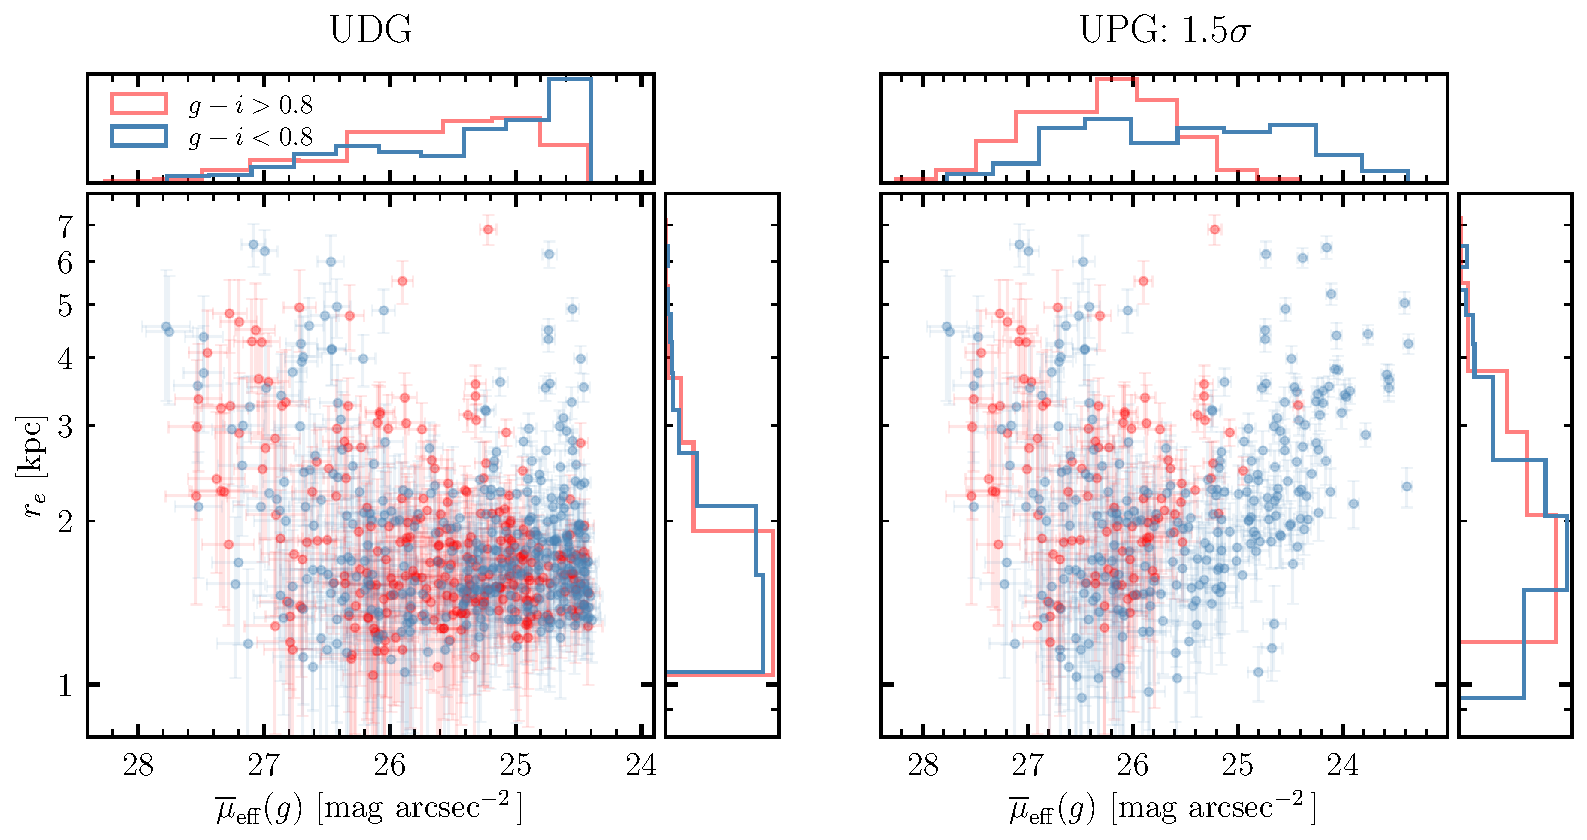
\includegraphics[width=1\linewidth]{udg_upg_sample.pdf}
	}
    \caption{The distribution of galaxies in the ultra-diffuse galaxy (UDG) sample (\textit{left}) and the ultra-puffy galaxy (UPG) sample (\textit{right}). The UDGs are galaxies with $r_e>1.5$ kpc and $\sbeff > 25.0\ \sbunit$. The UPGs is defined to be $1.5\sigma$ above the mass-size relation in \citet{ELVES-I}. We split the samples into two color bins and show them in red ($g-i>0.8$) and blue ($g-i<0.8$). The marginal histograms are not normalized to highlight the relative number of red and blue galaxies. Compared with the UDG sample, the UPG sample includes blue galaxies with surface brightness higher than the UDG cut ($\sbeff < 25\ \sbunit$) and excludes red galaxies at $25 < \sbeff < 26\ \sbunit$. We note that this plot is not corrected for background contamination.
    }
    \label{fig:udg_upg_re_mu}
\end{figure*}

We derive the stellar masses of UDGs and UPGs from the Spergel model fitting and a relation between color and mass-to-light ratio $M_{\star}/L$ from \citet{Into2013}:
\begin{align*}
&\log \left(M_{\star} / L_{g}\right)=1.774\,(g-r)-0.783, \\
&\log \left(M_{\star} / L_{g}\right)=1.297\,(g-i)-0.855.
\end{align*}
Because we have both $g-r$ and $g-i$ color available from the model fitting, we use the average of the $M_{\star}/L$ derived from the two colors for calculating stellar mass. We assume the solar absolute magnitude in $g$-band to be 5.03 \citep{Willmer2018}. 

\subsection{Background contamination}\label{sec:bkg}
The major weakness of LSBG searches in imaging data is that distance information is typically unknown. Although we have matched LSBGs to MW analogs by proximity, the physical affiliation of LSBGs to the host is not guaranteed. As a result, a certain fraction of galaxies in our UDG and UPG sample might just be foreground or background galaxies that fall within the virial radius of the host in projection. Given the volume probed by our search, contamination is most likely to be dominated by background galaxies. We estimate the contamination fraction as follows. The methodology is to study the number of those LSBGs that mimic UDGs and UPGs by randomly matching LSBGs to our MW hosts.

We randomly select a continuous patch of sky of 24 deg$^{2}$ in HSC PDR2. Then we perform the same deblending and modeling steps for the 2,707 LSBGs detected in this region. We also removed objects that are already in our UDG sample, and we did visual inspection to further remove spurious objects. In the end, there are 480 LSBGs representing a population of possible contaminants. Next, because both UDG and UPG are defined based on physical size, we randomly associate the 480 LSBGs to the hosts of our UDGs (UPGs). Then we calculate a physical size for each LSBG and classify an LSBG as a ``fake`` UDG (or UPG) if it satisfies the definition. We repeat such random matching for 200 times. In the end, we obtain 11,458 fake UDGs and 11,867 fake UPGs. These UDGs and UPGs are ``fake'' only in the sense of being associated with random MW hosts. 

In this way, the number density of fake UDGs is estimated to be $S_{\rm UDG} = 1.94\pm0.03\ \mathrm{deg}^{-2}$, and the number density of fake UPGs is $S_{\rm UPG} = 2.12\pm0.03\ \mathrm{deg}^{-2}$. The catalogs of fake UDG and UPGs are also available online\footnote{\url{https://github.com/AstroJacobLi/kuaizi/tree/master/data}}. Using the number densities and the probed area of our survey, we calculate the contamination fraction for both the UDG and UPG samples. For the UDG sample, we find $f_{\rm contam}^{\rm UDG} \approx 16\%$; for the UPG sample, the contamination fraction is $f_{\rm contam}^{\rm UPG} \approx 20\%$. We take the contamination fraction into account when calculating the abundance, size distribution, radial distribution of UDGs and UPGs in Section \ref{sec:results}. We note that we do not apply any background correction in Figure \ref{fig:mass_size} and Figure \ref{fig:size_distribution}.

One of the main goals of this paper is to study the star-forming properties of UDGs and UPGs in MW analogs. The star formation rate of galaxies can be indicated by their broad-band colors, and we use color to calculate the quenched fraction of UDGs and UPGs (see \S \ref{sec:quench} for more discussion). However, background contaminants affect the color distribution of the UDG (UPG) sample, thus affect the calculated quenched fraction. If the fake UDGs (UPGs) have different properties from the real ones, we can use these information to derive a possibility for an object of being a real UDG (UPG). % If the fake UDGs (UPGs) span a different region from the true UDGs in the observable space, we can use these observables to assign weights to each object in our UDG sample indicating the possibility of being a true UDG. 
Indeed, we find that the $g-i$ color distribution of the fake UDG (UPG) sample is bluer than that of the true UDG (UPG) sample, which motivates us to assign importance weights based on the $g-i$ color. We first compute the normalized histograms of $g-i$ colors (denoted as $\lambda_k$ at the $(g-i)_{k}$ bin) for both true UDG and fake UDG samples. Then we multiply $f_{\rm contam}^{\rm UDG}$ with the histogram of fake UDG sample ($\lambda_k^{\rm fake}$) such that the histogram sums up to the average contamination fraction. The weights of UDGs in color bin $(g-i)_k$ is estimated to be $w_k = \max\,(1 - f_{\rm contam} \lambda_k^{\rm fake} / \lambda_k^{\rm true}, 0)$. This weight stands for a possibility of not being a contaminant. The weights of UPGs are assigned following the same procedure. We find this color-based contamination subtraction scheme is sufficient for this work since the contamination fraction is small. Our main results shown in Section \ref{sec:quench} are robust against contamination subtraction. 


\section{Results}\label{sec:results}
In this section, we present statistical analysis of UDGs and UPGs associated with MW analogs at $0.01 < z < 0.04$.

\subsection{UDG and UPG on the mass-size plane}\label{sec:mass-size}
\begin{figure*}
	\vbox{ 
		\centering
		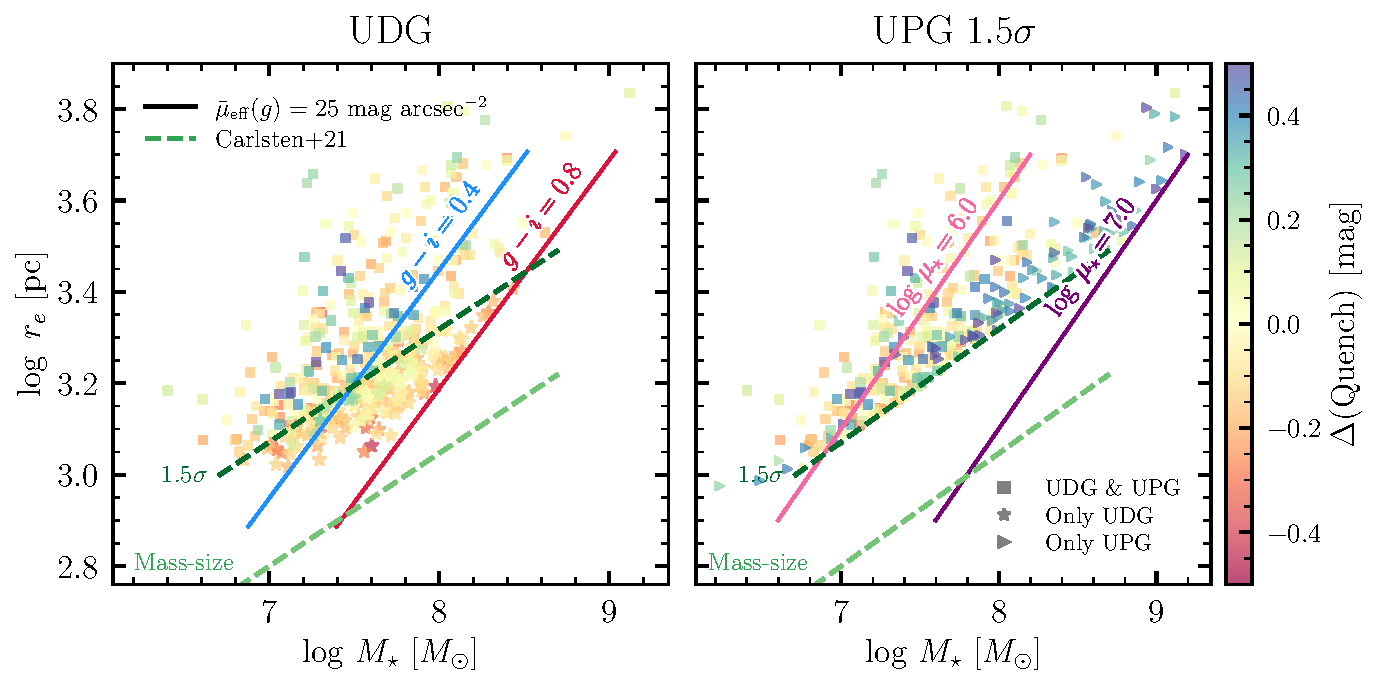
\includegraphics[width=1\linewidth]{mass_size_plane.pdf}
	}
    \caption{The distributions of the UDG and UPG sample on the mass-size plane. The data points are color-coded by the distance to the quenching color cut. Squares are those galaxies satisfying both UDG and UPG definition, stars (triangles) are those only satisfying UDG (UPG) definition.
    We plot the average mass-size relation (light green) and $1.5\sigma$ above the average relation (dark green) as dashed lines for reference. In the left panel, we show the constant surface brightness line as solid lines by assuming two different $g-i$ colors. Galaxies falling between these two lines are mostly red and quenched because blue UDGs have too be very large in size to satisfy the surface brightness criterion. This hard surface brightness cut makes the UDG quenched fraction high. The constant surface mass density lines in the right panel might provide us new ways to define diffuse dwarf galaxies.
    }
    \label{fig:mass_size}
\end{figure*}
Since we propose a new subset of LSBGs as UPG, some intuitions on the UPG population and the difference between UDG and UPG are needed. In order to build a more comprehensive understanding on our UDG and UPG sample, we show their distributions on the mass-size plane in Figure \ref{fig:mass_size}. In the left panel, UDGs that are also classified as UPGs are shown in squares, while UDGs that do not satisfy UPG definition are marked as stars. In the right panel, triangles correspond to UPGs that are not classified as UDGs. To orient the readers on the mass-size plane, we also display the average mass-size relation derived from the satellites of MW analogs in the Local Volume \citep{ELVES-I} as the light green dashed line. The darker green line shows $1.5\sigma$ above the average mass-size relation assuming the scatter of the mass-size relation to be $\sigma=0.181$ dex \citep{ELVES-I}. Because UDGs are defined to have $r_e > 1.5$ kpc and $\sbeff > 25.0\ \sbunit$, we see a hard cut on size and surface brightness in the left panel. We also see that UPGs are all above the $1.5\sigma$ line by construction. Comparing the two panels, we find that the UDG sample includes a number of galaxies below $1.5\sigma$ line (highlighted as stars), but also lose a few low-mass galaxies with sizes smaller than 1.5 kpc. UDGs below $1.5\sigma$ line have sizes larger than 1.5 kpc, but they are not large enough for their stellar masses. It is also noticeable that the UPG sample has a few galaxies with $M_\star > 10^{8.5}\ M_\odot$ which have surface brightness brighter than $25.0\ \sbunit$. 
% As a consequence, the size distribution of UPGs at the smaller end is suppressed as shown in Fig. \ref{fig:size_distribution}.

As we will introduce in Section \ref{sec:quench}, we use a color cut $(g-i)_{Q}$ to separate galaxies with active star formation from quiescent ones. Here we define $\Delta(\mathrm{Quench}) = (g-i) - (g-i)_{Q}$ as an indicator for the star formation rate of the galaxy. Higher $\Delta(\mathrm{Quench})$ indicates that the galaxy is actively star-forming, whereas lower $\Delta(\rm Quench)$ means the galaxy has lower star formation rate. We color-code the galaxies in Figure \ref{fig:mass_size} with $\Delta(\mathrm{Quench})$. UDGs below the $1.5\sigma$ line have near zero or negative $\Delta(\mathrm{Quench})$, indicating that the UDG sample includes plenty of quenched galaxies compared with the UPG sample. Instead, the UPG sample is comprised of many star-forming galaxies at the high-mass end. 

% In Figure \ref{fig:mass_size}, we also show constant surface brightness lines in the left panel and constant mass surface density in the right panel. We will discuss how the definition of UDG could bias the quenched fraction later in Sec. \ref{sec:discussion}. 

\jiaxuan{@Jenny: any other things to mention in this section?}

\subsection{Abundance of UDGs and UPGs}\label{sec:n_udg}

\begin{figure*}
	\vbox{ 
		\centering
		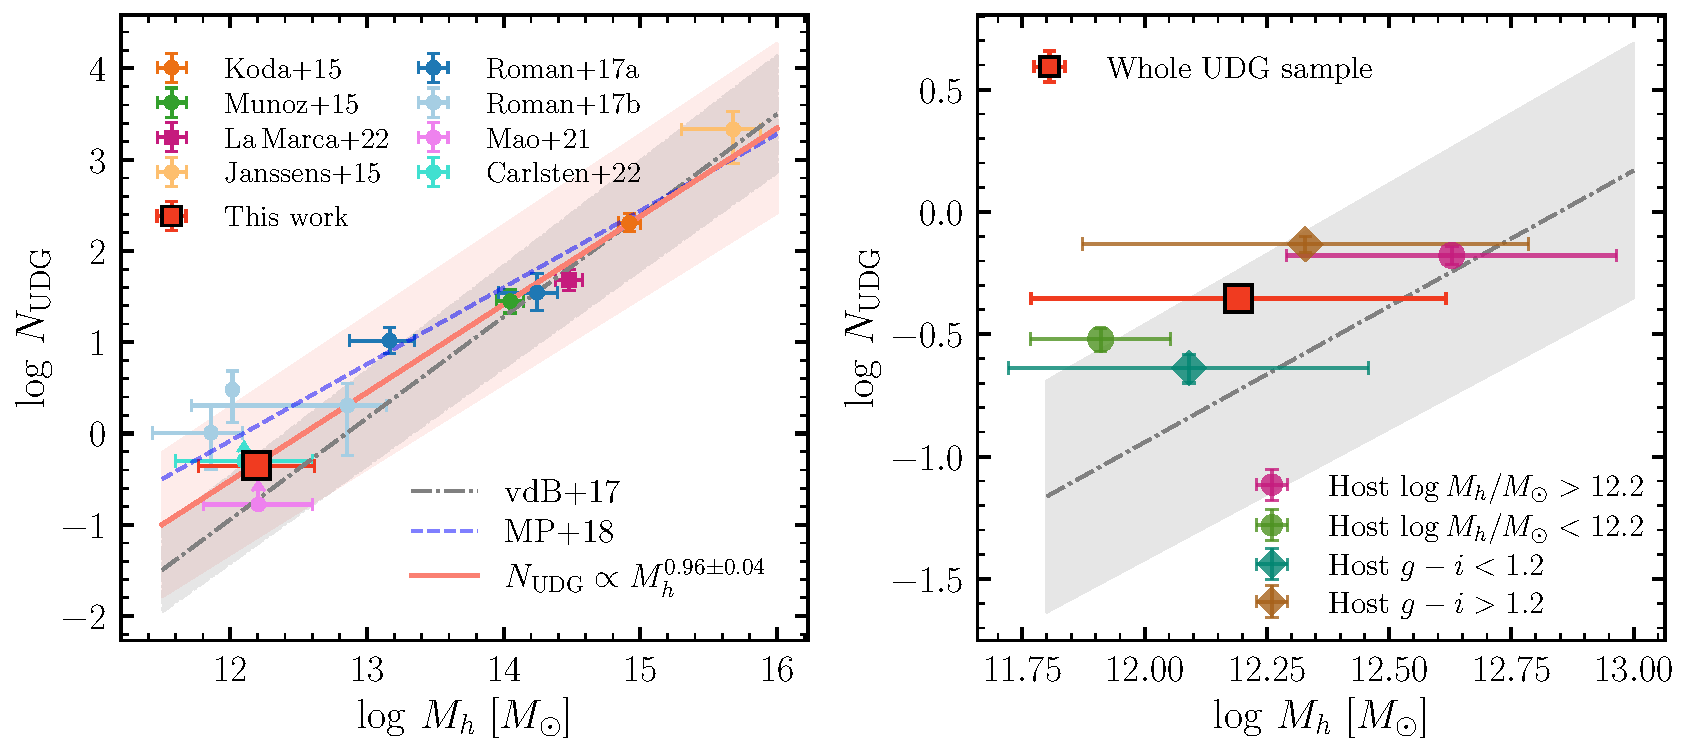
\includegraphics[width=1\linewidth]{N_UDG_host_mass.pdf}
	}
    \caption{The abundance of UDGs as a function of host halo mass. \textit{Left}: We compile the UDG abundance measurements from literature covering a wide range of host mass. The UDG abundance of our work $N_{\rm UDG} = 0.76\pm 0.04$ is shown as red square, the power-law relation from \citet{vdBurg2017} is shown in gray, and our fitting result is shown in pink. Our UDG abundance is consistent with ELVES but significantly higher than that in SAGA. After including more measurements at the lower halo mass end, the power-law is shallower than the relation reported in \citet{vdBurg2017}. \textit{Right}: We split the UDG sample into bins based on the host halo mass (triangles) and $g-i$ color (pentagons). The UDG abundance is higher for more massive host and redder host. }
    \label{fig:n_udg}
\end{figure*}

As demonstrated by many previous studies \citep[e.g.,][]{vdBurg2016,vdBurg2017,Roman2017a}, the average number of UDGs per host scales with host halo mass. While much literature focuses on finding UDGs in clusters and large groups, there are fewer constraints on the UDG abundance at the lower halo mass end. In this section, we calculate the UDG and UPG abundances of MW analogs, and compare with other surveys.

We define the UDG (UPG) abundance as the average number of UDGs (UPGs) per host galaxy. In our UDG sample, there are 412 UDGs associated with 258 hosts. After correcting for background contamination (see \S \ref{sec:bkg}) and completeness (see \S \ref{sec:completeness}), the UDG abundance of MW analogs is $N_{\rm UDG} = 0.76\pm 0.04$ per host. The UPG abundance in our sample is $N_{\rm UPG} = 0.61\pm 0.04$ per host. Here we neglect the fact that the number of satellites contained within the virial sphere is different from the number of satellite within a projected cylinder with virial radius (the so-called deprojection factor, \citealt{vdBurg2017}).


We compare our UDG abundance with other surveys focused on MW analogs. In the SAGA survey \citep{SAGA-II}, 6 satellite galaxies (out of 127 spectroscopy-confirmed satellites around 36 MW analogs) satisfy the definition of UDG. Therefore the UDG abundance in \citet{SAGA-II} is about $N_{\rm UDG,\, SAGA} \approx 0.17\pm0.07$. In the ELVES survey \citep{CarlstenELVES2022}, there are 15 satellites (out of 404 satellites associated with 30 MW analogs) satisfying the UDG definition, leading to a UDG abundance of $N_{\rm UDG,\, ELVES} \approx 0.50\pm0.13$. \citet{Roman2017b} identified 11 UDGs around three galaxy groups in the IAC Stripe 82 Legacy Survey \citep{Fliri2016}. Because both SAGA and ELVES select satellites based on distance measurements and do not correct for completeness, we interpret their UDG abundances as lower limits. We note that \citet{Roman2017b} do not estimate the background contamination fraction and correct for completeness. We plot the UDG abundances of these surveys in the left panel of Figure \ref{fig:n_udg}, together with the results for larger galaxy groups and clusters \citep{Koda2015,Munoz2015,Roman2017a,Roman2017b,Janssens2017,vdBurg2017}. Among these studies, only \citet{vdBurg2017} applies a background subtraction and completeness correction to the raw counts.
% In the Auriga simulations, \citet{Liao2019} find $N_{\rm UDG,\,Auriga}=1.27\pm 1.06$ for UDGs in MW-mass hosts. 
The power-law regression result from \citet{vdBurg2017} $N_{\rm UDG} \propto M_h^{1.11\pm 0.07}$ is shown in gray. The UDG abundance of this work is highlighted as the red square. As shown in Figure \ref{fig:n_udg}, the scatter in the $N_{\rm UDG}-M_h$ relation gets larger at the lower halo mass end. Our UDG abundance is similar to the value in ELVES survey, but much higher than the value from SAGA. This might be explained by the different photometric depth of data used. As pointed out by \citet{CarlstenELVES2022,Font2022}, SAGA survey reaches a surface brightness depth of $\sbeffr\approx 25\ \sbunit$, which is $\sim 2.5\ \sbunit$ shallower than the ELVES survey and this work. It is probable that SAGA missed a significant fraction of red and lower surface brightness galaxies. Our UDG abundance is marginally higher than the prediction from \citet{vdBurg2017} but is still consistent considering the large scatter of the power law. 

Taking all data points from literature (as shown in Figure \ref{fig:n_udg}), we use the orthogonal distance regression (ODR) to fit a power-law between $N_{\rm UDG}$ and host halo mass $M_h$ and find $N_{\rm UDG} \propto M_h^{0.96\pm 0.04}$, shown as the red dashed line in Figure \ref{fig:n_udg}. The slope of the power law is shallower than \citet{vdBurg2017} ($\beta=1.11\pm0.07$) but still steeper than \citet{Roman2017b} ($\beta=0.85\pm0.05$). \citet{ManceraPina2018} survey eight clusters and find sublinear power laws. Since most individual studies do not have a statistical estimation for background contamination and completeness, the UDG abundances for large groups should be interpreted as lower limits. If completeness is applied, it is possible that the slope $\beta$ will be steeper than what we are showing in Figure \ref{fig:n_udg}. We also note that many studies do no consider measurement bias and uncertainty, which makes the comparisons more difficult.

In the right panel of Figure \ref{fig:n_udg}, we split the UDG sample into different bins based on their host halo mass (shown as triangles) and host color (shown as pentagons). We find that the UDG abundance is slightly higher for hosts with higher halo mass and redder color, but the trend is stronger with host color. 
% Since there are not many data sets available for us to derive UPG abundances, we only take the ELVES results \citep{CarlstenELVES2022} and obtain $N_{\rm UPG} = $

Another interesting quantity is the fraction of UDGs (UPGs) out of all satellites in a group or cluster. This fraction represent how efficient an environment is at producing diffuse galaxies. We denote this quantity as UDG (UPG) fraction hereafter, which characterizes the tail of the size distribution of satellites. In order to calculate this fraction, we assume that MW analogs have $\sim 5$ satellites with $M_\star > 10^{6.5}\ M_\odot$ \citep{CarlstenELVES2022}. This lower limit of stellar mass is roughly our detection limit (see Fig. \ref{fig:mass_size}). Then for our samples, the UDG (UPG) fraction is $f_{\rm UDG} \approx 0.15$ and $f_{\rm UPG} \approx 0.12$. \jiaxuan{In ELVES, there are 25 UDGs and 27 UPGs out of xxx satellites, so $f_{\rm UDG} \approx xxx$ and $f_{\rm UPG} \approx xxx$. The ELVES results are consistent with ours.} We also compare our results with the Virgo cluster. Taking the data from the Next Generation Virgo Cluster Survey (NGVS, \citealt{Ferrarese2020}), there are 15 UDGs and 24 UPGs out of 404 identified satellites without completeness correction. Thus their UDG (UPG) fraction is $f_{\rm UDG,\  Virgo}=0.04$ and $f_{\rm UPG,\ Virgo} = 0.06$. However, we note that \citet{Ferrarese2020} only survey the central 4 deg$^2$ of the Virgo cluster, which probably biases the UDG (UPG) fraction. A more systematic comparison on UDG (UPG) fraction in different environments is needed in the future. 

\subsection{Size distribution}\label{sec:size_distr}

\begin{figure*}
	\vbox{ 
		\centering
		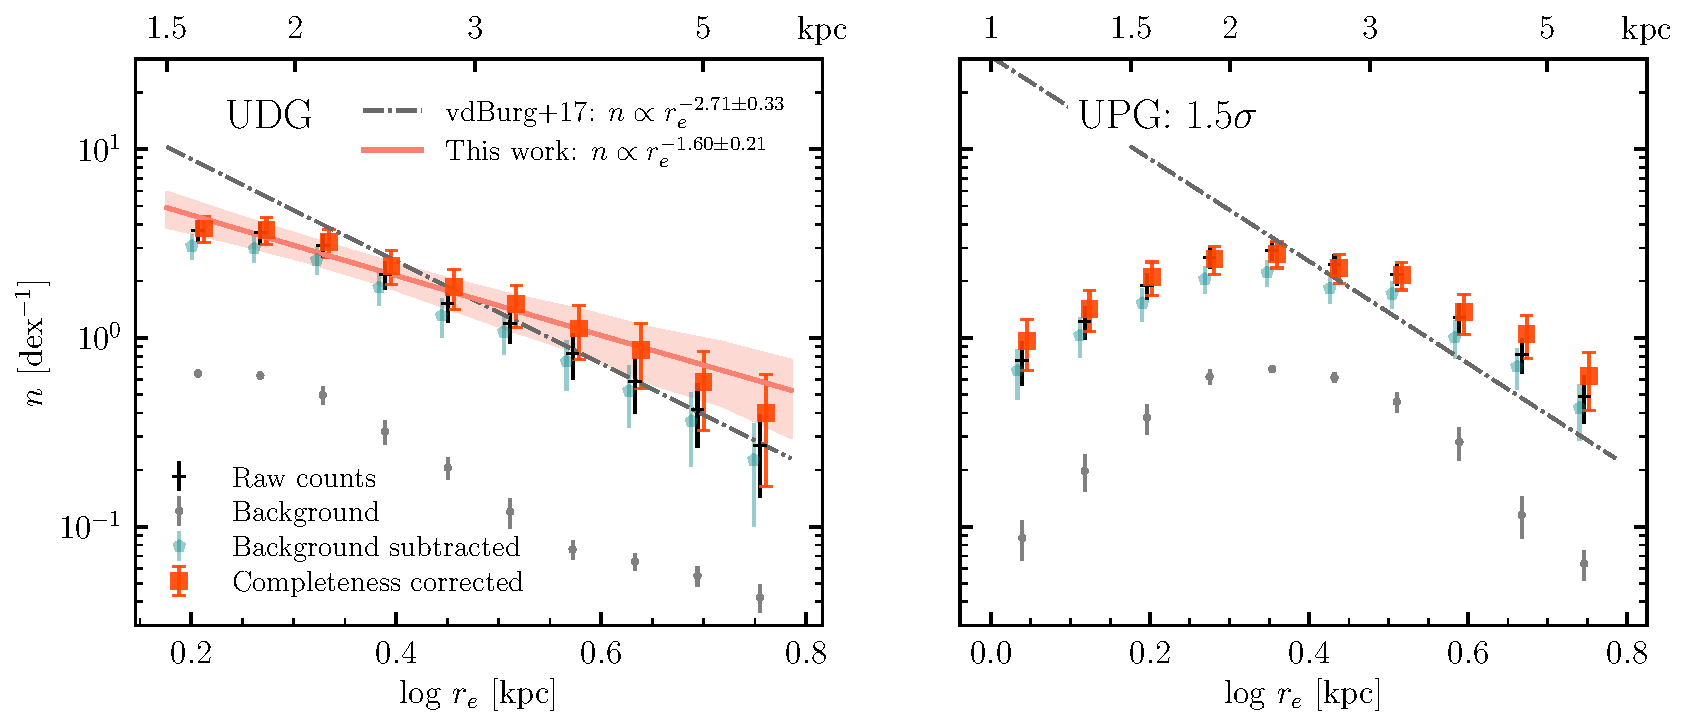
\includegraphics[width=1\linewidth]{size_distribution.pdf}
	}
    \caption{The size distribution of UDGs (\textit{left}) and UPGs (\textit{right}). The contribution from the background contaminants (gray dots) are subtracted and the completeness has been corrected. We fit a power law to the size distribution of UDGs and get a power law shallower than that from \citet{vdBurg2016,vdBurg2017}. We find that the power law slope increases as the average halo mass increases. It is possible that denser environments provide stronger tidal forces thus produce more smaller UDGs. The UPG size distribution is suppressed at the smaller size end because small galaxies are not $1.5\sigma$ above the mass-size relation.
    }
    \label{fig:size_distribution}
\end{figure*}

The size distribution of UDGs is an important topic since it has been used to test UDG formation scenarios \citep[e.g.,][]{Amorisco2016,vdBurg2017}. In this section, we calculate the size distribution of our UDG and UPG sample. First of all, we take the fake UDGs in random fields (\S \ref{sec:bkg}) and calculate their size distribution as a proxy for background contamination, shown as the gray dots in the left panel of Figure \ref{fig:size_distribution}. For each host, we calculate the raw size distribution of the associated UDGs (black dots), and we multiply the background size distribution by the virial area of the host and subtract it from the raw size distribution. Then we combine the UDG size distributions for all hosts together, and correct for completeness (red squares). Since the stellar masses of the hosts in our sample are quite similar, we do not weight each host according to their masses. The error shown in Figure \ref{fig:size_distribution} takes both Poisson error and the measurement error in size into account.

We find that the UDG size distribution roughly follows a power law. We fit a power law relation to our UDG size distribution and get $n\propto r_e^{-1.60\pm0.21}$. This is shallower than the power law presented in \citet{vdBurg2016} ($n\propto r_e^{-3.40\pm0.19}$) and \citet{vdBurg2017} ($n\propto r_e^{-2.71\pm0.33}$, shown as gray dash-dotted lines in Figure \ref{fig:size_distribution}). We also split the UDG sample based on their host stellar masses and distance to hosts, but consistently find shallow power-laws with index $\sim -1.6$. In particular, we do not find significant change in the size distribution as UDGs (UPGs) get closer to their hosts. Among others, \citet{vdBurg2016} focus on large galaxy clusters and find a very steep slope, \citet{vdBurg2017} includes less-massive groups and the slope is less steep. Combined with our findings, it might be possible that dense environment produces more smaller UDGs. As we will discuss in Section \ref{sec:discussion}, cluster environments provide stronger tidal fields and thus are more efficient on producing smaller UDGs due to tidal stripping. 

We also show the size distribution of UPGs in the right panel of Figure \ref{fig:size_distribution}. As we shown in Figure \ref{fig:mass_size}, the UPG sample does not have those galaxies below the $1.5\sigma$ line but larger than 1.5 kpc. Therefore, for a given mass, many small UDGs are not in the UPG sample since their sizes are not extreme on the mass-size plane. As a consequence, the size distribution of UPG sample is suppressed at the smaller size end. 

\subsection{Radial distribution}\label{sec:radial_distr}

\begin{figure*}
	\vbox{ 
		\centering
		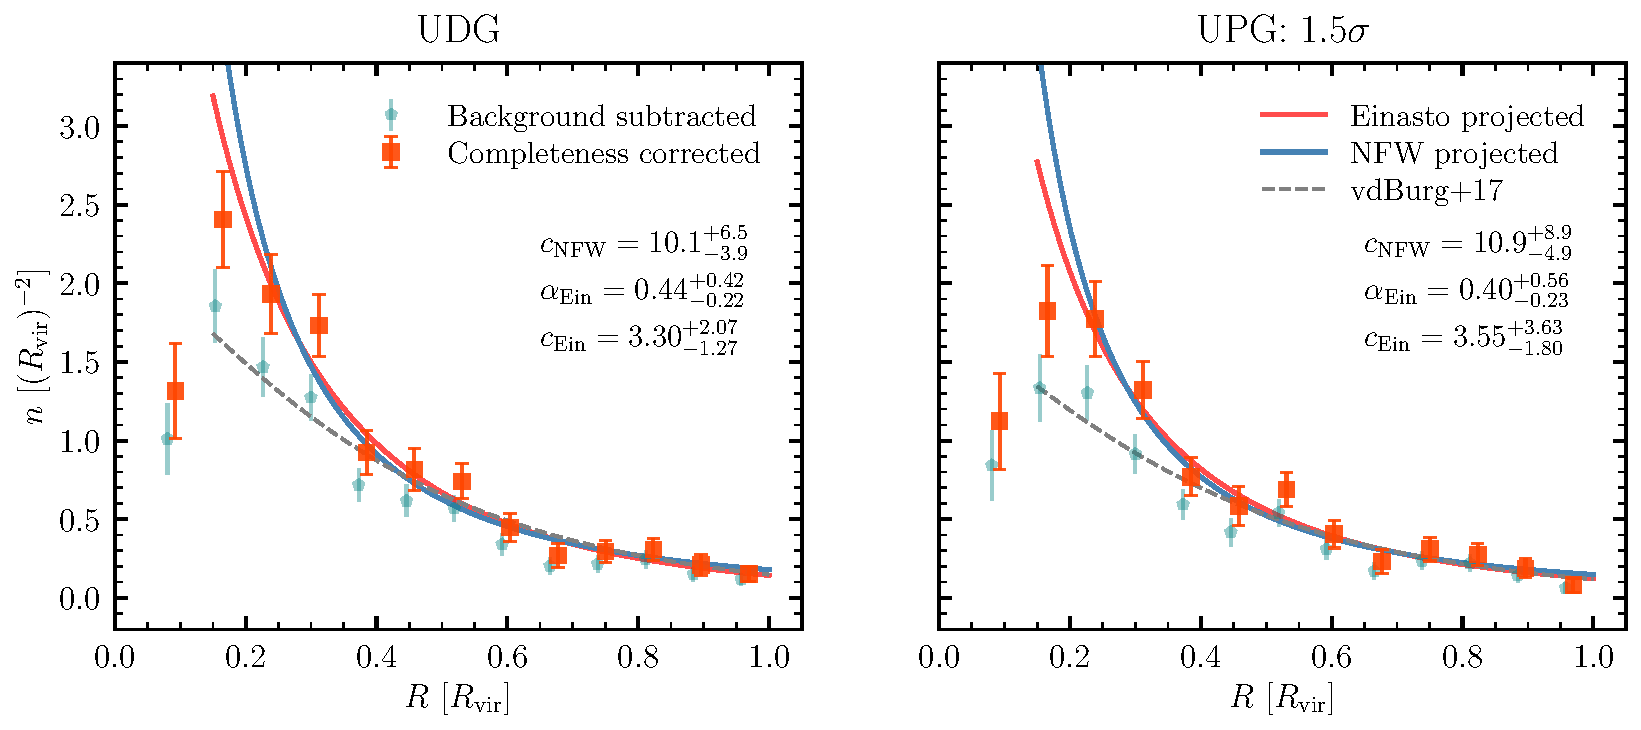
\includegraphics[width=1\linewidth]{radial_distribution.pdf}
	}
    \caption{The radial distributions of UDGs (\textit{left}) and UPGs (\textit{right}). We subtract the background contamination (shown in teal) and correct for completeness in each radial distance bin (shown in red). We fit the projected NFW and Einasto profiles to the radial distributions and find good fits for both profiles. The radial distributions of UDGs and UPGs are similar in shape. The best-fit NFW concentrations is consistent with a MW-mass halo, whereas the best-fit Einasto profiles have smaller concentration than MW-mass halos.}
    \label{fig:radial_distribution}
\end{figure*}


The radial distribution of UDGs around the hosts has been used to test various UDG formation theories \citep[e.g.,][]{Tremmel2020}. In \citet{vanDokkum2015}, UDGs are not found within 300 kpc from the cluster center, hinting that UDGs might not survive in such a dense environment. \citet{vdBurg2016,ManceraPina2018} also found that the number of UDGs is depleted near the center of clusters. In \citet{vdBurg2016}, the radial distribution of UDGs in cluster environments roughly follows a projected Einasto profile \citep{Einasto1965}. In this subsection, we derive the radial distribution of UDGs and UPGs in our sample and discuss possible implications.

We calculate the radial distribution as follows. For each host, we count the number of UDGs (UPGs) in each radial bin scaled by $R_{\rm vir}$ and calculate the number density of UDGs (UPGs) within each radial annulus. We subtract the contribution of background contaminants based on the background contamination density (\S \ref{sec:bkg}) and the angular area occupied by the host. Then we average over all hosts and correct for the completeness, as shown in Figure \ref{fig:radial_distribution}. Red squares are the number of UDGs (UPGs) per radial bin, and the error includes Poisson error, background subtraction error, and completeness error. The radial distributions of both UDGs and UPGs turn over around $R=0.2\,R_{\rm vir}$. It is known that the detection can be more incomplete as it gets closer to the host due to the blending between UDG and the host galaxy or due to sky subtraction issues. Although we have corrected the completeness for each object based on their size and surface brightness, it is still possible that our completeness does not fully characterize the radial dependence of completeness. As we mentioned above, it is also possible that UDGs and UPGs are depleted because of tidal disruption. 

We fit the radial distributions of UDGs (UPGs) with the projected NFW and Einasto profiles for $R > 0.2 R_{\rm vir}$. The Einasto profile introduces an extra ``shape'' parameter $\alpha$ and has been argued to be a better description to the dark matter halo profiles \citep[e.g.,][]{Navarro2004,Gao2008,Navarro2010,Dutton2014}. The Einasto profile also makes concentration estimates less sensitive to the radial range fitted. The best-fit NFW (blue) and Einasto (red) profiles are shown in Figure \ref{fig:radial_distribution} as solid lines. The best-fit Einasto profile from \citet{vdBurg2016} is shown as the dashed gray line.

Compared with \citet{vdBurg2016}, there are more UDGs at smaller radial distances in our sample, thus the UDG radial distribution is more concentrated although we exclude $R < 0.2\ R_{\rm vir}$. Unlike \citet{vdBurg2016}, we find that both NFW and Einasto could describe the radial distribution of UDGs (UPGs) quite well. The concentration of the best-fit NFW profile is $c_{\rm NFW, UDG} = 10.1^{+6.5}_{-3.9}$ for UDGs and $c_{\rm NFW, UPG} = 10.9^{+8.9}_{-4.9}$ for UPGs. The best-fit Einasto profile has $\alpha_{\rm Ein, UDG} = 0.44^{+0.42}_{-0.22},\ c_{\rm Ein, UDG} = 3.30^{+2.07}_{-1.27}$ for UDGs and $\alpha_{\rm Ein, UPG} = 0.40^{+0.56}_{-0.23},\ c_{\rm Ein, UPG} = 3.55^{+3.63}_{-1.80}$ for UPGs. The radial distribution profiles of UDGs and UPGs are found to be very similar in shape. Our best-fit Einasto profiles have lower $\alpha$ and higher concentration compared with \citet{vdBurg2016} where they have $\alpha_{\rm Ein, UDG} = 0.92^{+0.08}_{-0.18},\ c_{\rm Ein, UDG} = 1.83^{+0.13}_{-0.12}$.

According to the concentration-mass relation of dark matter halos, the concentration of MW-like halo is $c_{\rm NFW} \sim 10$ \citep[e.g.,][]{Bullock2001,Duffy2008,Dutton2014,Diemer2019}. Therefore, if assuming an NFW profile, the UDGs and UPGs follow the underlying dark matter distribution of the host. However, the Einasto shape parameter for a MW-like halo is $\alpha\sim 0.15$ at $z=0$ and its concentration is $c\sim 8-10$. \citep{Gao2008,Dutton2014}. Comparing with this, the best-fit Einasto profiles for UDGs and UPGs are in tension with MW dark matter profile. We notice that the errors of the best-fit parameters are large due to the sample size and also the fact that concentration is most sensitive to data at smaller radial distances which are excluded in the analysis. Therefore, we consider the UDG (UPG) radial distribution to be consistent with the dark matter distribution of the host at a $2\sigma$ level. Nevertheless, a larger, cleaner, and more complete sample is needed to better constrain the radial distributions. 


\subsection{Quenched fraction}\label{sec:quench}

\begin{figure*}
	\vbox{ 
		\centering
		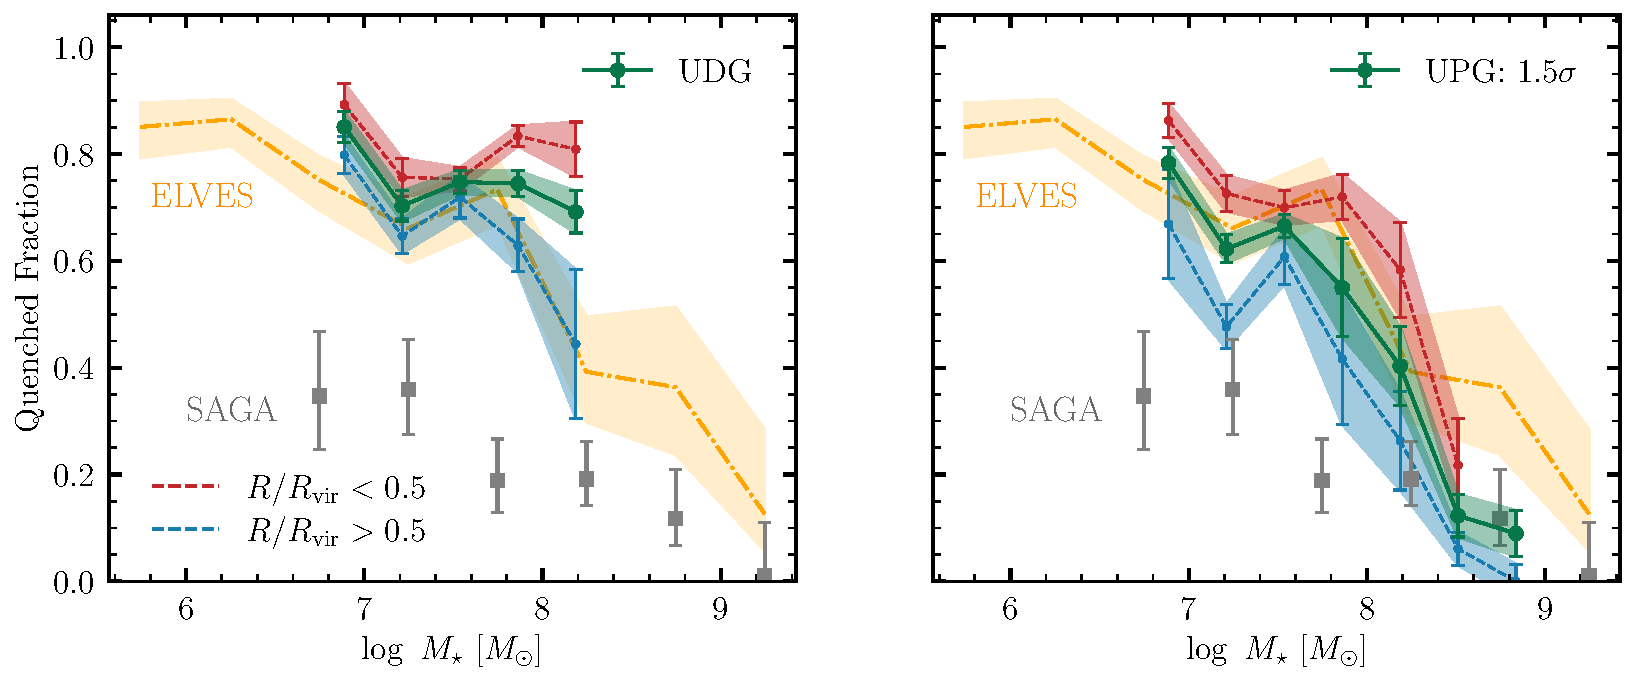
\includegraphics[width=1\linewidth]{quenched_frac_dist2host.pdf}
		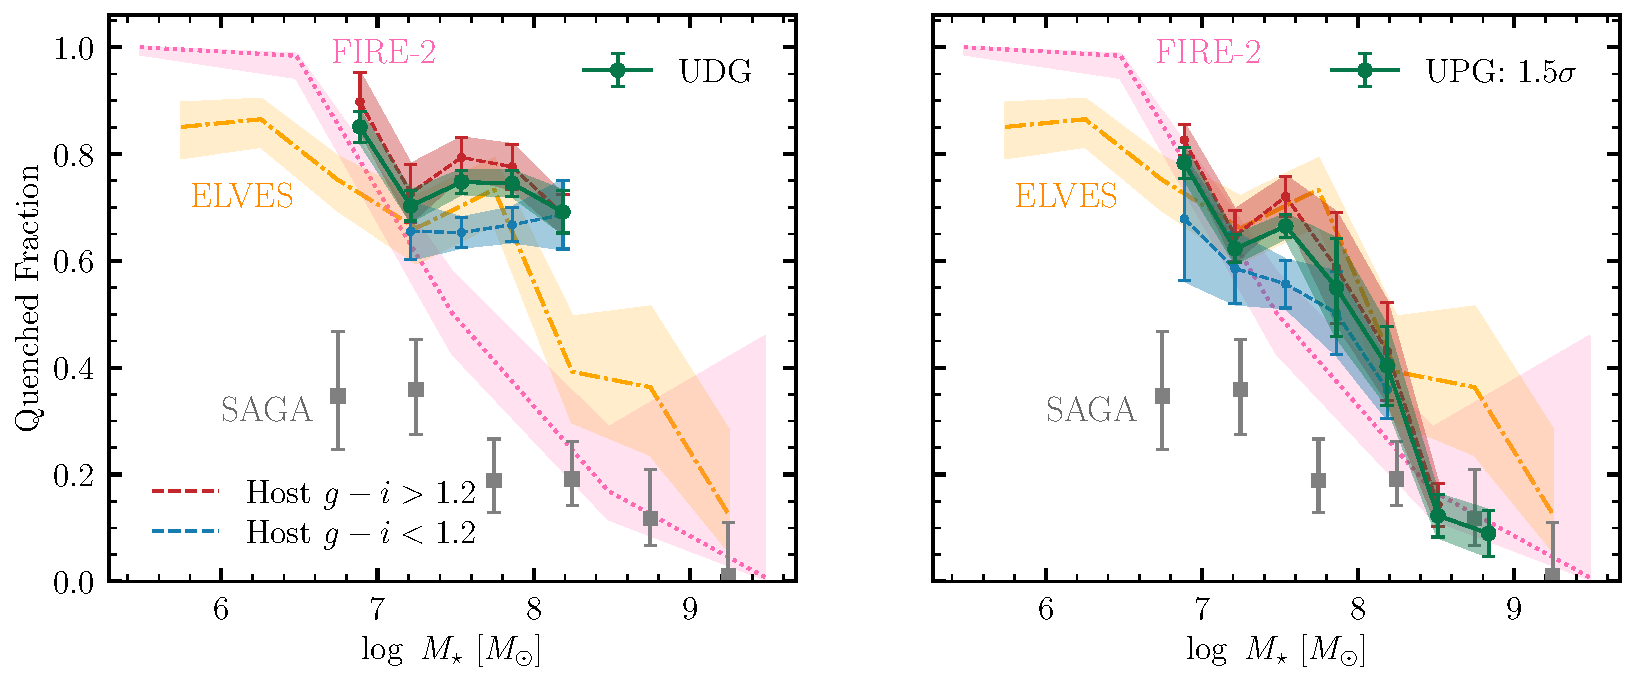
\includegraphics[width=1\linewidth]{quenched_frac_host_color.pdf}
	}
    \caption{The quenched fractions of UDGs (left panels) and UPGs (right) as a function of their stellar masses. The results for the whole sample are shown in green dots. The samples are further divided into bins based on the radial distance to the host (top panels) and host color (bottom panels), and are displayed in blue and red lines. We also overlie the results from Local Volume \citep[ELVES,][]{CarlstenELVES2022}, nearby Universe \citep[SAGA,][]{SAGA-II}, and simulations including ARTEMIS \citep{Font2022} and FIRE-2 \citep{Samuel2022}. The errors in this plot correspond to $1\sigma$ Bernoulli standard error. We find that UDGs have high quenched fraction and remains a constant across a decade in stellar mass. The quenched fraction of UPGs drops as increasing stellar mass, remarkably similar to that of normal satellites of MW analogs. The quenched fraction is larger for those associated to redder hosts and those that are closer to the host. }
    \label{fig:qfrac}
\end{figure*}

\begin{figure}
    \centering
    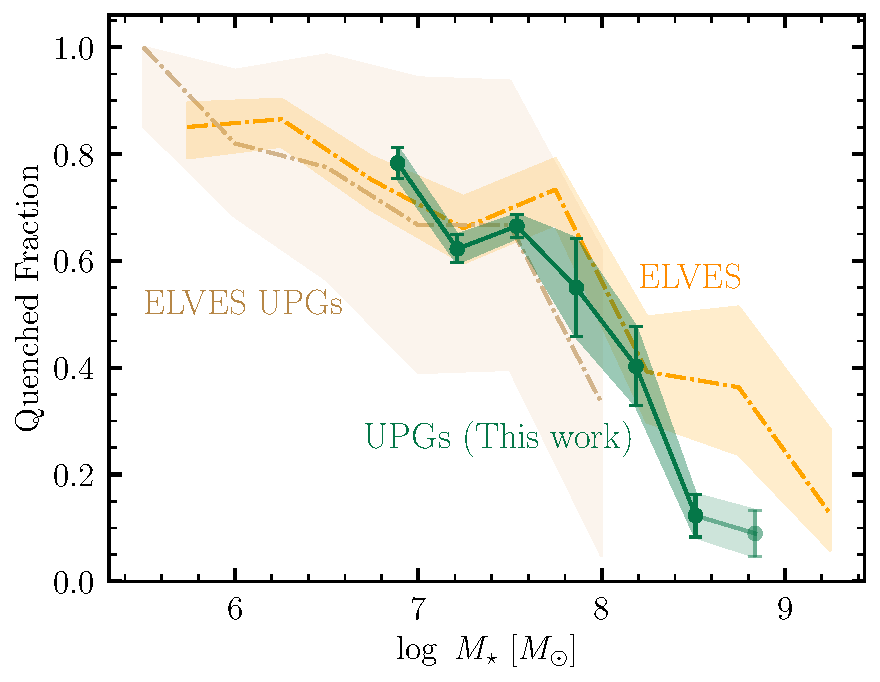
\includegraphics[width=1\linewidth]{quenched_frac_elves.pdf}
    \caption{A comparison on UPG quenched fractions with ELVES (Greene et al., in prep).}
    \label{fig:qfrac_upg_elves}
\end{figure}
The star-forming properties of UDGs and UPGs is an interesting subject given their diffuse stellar component and possible non-trivial formation history. In this section, we study the fraction of quenched UDGs and UPGs as a function of both stellar mass and their host properties. We defer the discussion on the implications of these results to Section \ref{sec:discussion}.

We refer to quenching as the cessation of star formation in galaxies. In principle, direct estimates for the instantaneous star formation rate (SFR) from UV or H$\alpha$ or estimations for the \ion{H}{1} gas are needed to define a quenched galaxy  population. As an example, the SAGA survey measures the H$\alpha$ equivalent width (EW) from spectra to define quenched satellites. There are also many studies probing \ion{H}{1} masses for MW and M31 satellites \citep[e.g.,][]{Grcevich2009,Spekkens2014,Putman2021}. However, these specific data sets are either not deep enough to probe our UDGs and UPGs, or they are very expensive to obtain and cover all the footprint of our sample. Therefore, we seek other indicators including integrated color and morphology to approximate star-forming properties. \citet{CarlstenELVES2022} visually inspected all satellites and classified them into early-type (red and smooth) and late-type (blue, asymmetric, clumpy). Using this sample, they find that a mass-dependent color cut $(g-i)_{Q} = -0.067\, M_V - 0.23$ could also divide the sample into early- and late-type that are nearly identical to the ones based on morphology. The derived quenched fractions based on morphology and color are very similar. Furthermore, \citet{Font2022} showed in simulations that this color cut effectively separates star forming galaxies from quenched ones. This makes the color cut more promising since their simulations are not fine tuned to match the observed properties of dwarfs. Since we do not visually inspect all UDGs and UPGs in our sample, we take the color cut from \citet{CarlstenELVES2022} to define our quenched galaxies: galaxies that are redder than $g-i > -0.067 M_V - 0.23$ are defined as quenched, whereas those bluer galaxies are thought to be star-forming. However, one caveat is that this criterion was derived from LV satellites in \citet{CarlstenELVES2022} and the bulk of them have higher surface brightness and less extended than our UDGs and UPGs. It is not guaranteed that the same color cut would work in our regime. \footnote{\jiaxuan{Add some robustness tests, such as ``Changing the intercept of the color cut to -0.28 makes the overall quenched fraction higher, but does not change the trend of quenched fraction as a function of stellar mass.''}}

We derive $V$-band apparent magnitude following $V = g - 0.5784\, (g - r) - 0.0038$\footnote{This relation was derived for SDSS filters. We neglect the small difference between SDSS and HSC filter systems. \url{http://classic.sdss.org/dr4/algorithms/sdssUBVRITransform.html\#Lupton2005}} and convert it to absolute magnitude $M_V$. For UDGs (UPGs) in each stellar mass bin, we calculate the fraction of quenched galaxies, but both denominator and numerator are weighted by the weights $w_k$ assigned in Section \ref{sec:bkg} to mitigate the impact of background contamination on quenched fractions. We also applied completeness correction. 
% We notice that such statistical background subtraction actually raise the quenched fraction since it reduces the impact of contaminants that are bluer in color.

\jiaxuan{Also describe that we don't see a redshift trend. Null trend in redshfit also attest that our sample is not subjecct to background contamination.}
describe the quenched fraction in percentage, e.g., half of them are quenched at 1e8. 

In Figure \ref{fig:qfrac}, the green lines show the quenched fractions $f_q$ as a function of stellar mass for the whole UDG (\textit{left}) and UPG (\textit{right}) samples, and the error bars correspond to the $1\sigma$ Bernoulli standard error. The quenched fraction of UDGs is high ($\sim 0.7$) over $6.8 < \log\ M_\star/M_\odot < 8.5$ and weakly depends on the stellar mass. On the contrary, as increasing stellar mass, the quenched fraction of UPGs drastically decreases from $f_q \approx 0.8$ at $M_\star = 10^{6.8}\ M_\odot$ to $f_q \approx 0.1$ at $M_\star = 10^{8.5}\ M_\odot$. We further divide the sample based on the projected radial distance to the host $R/R_{\rm vir}$ (top panels) and the host $g-i$ color (bottom panels). As shown in the top panels in Figure \ref{fig:qfrac}, we find that UDGs (UPGs) that are closer to the host have a higher quenched fraction. The average difference on quenched fractions between the two radial bins is $\sim 0.1$ for UDG and $\sim 0.2$ for UPG. This trend is expected because the density of CGM is higher when it is closer to the host and thus quenches the UDGs (UPGs) via ram pressure stripping more efficiently. The tidal stripping is also stronger as satellites get closer to the host. From the bottom panels in Figure \ref{fig:qfrac}, we find that UDGs (UPGs) hosted by redder hosts also have a higher quenched fraction. The difference on quenched fraction between the two host color bins is $\sim 0.2$ for UDGs. But for UPGs, it seems that the host color impacts less than the distance to the host on the quenched fraction. This result might hint at ``galaxy conformity'', which refers to the fact that late-type hosts tend to have more late-type satellites \citep{Weinmann2006}. We also split the samples based on host stellar mass, but do not find a significant difference in quenched fractions. (echo Jenny's paper)

We compare the quenched fractions of UDGs and UPGs with satellites of MW-mass hosts in the Local Volume (ELVES), in nearby Universe (SAGA), and in numerical simulations. The quenched fractions from ELVES is shown in orange dashed lines, while SAGA results are shown as gray squares. The quenched fraction from ELVES and SAGA used the same color cut to define quenched galaxies as we do (see \citealt{CarlstenELVES2022}). SAGA quenched fractions are lower than ELVES arguably because SAGA survey is not sensitive to galaxies below $\sbeffr = 25\sbunit$ \citep{Font2022}. We also overlie the quenched fraction from ARTEMIS \citep[purple lines,][]{Font2022} and FIRE-2 \citep[pink dotted lines][]{Samuel2022} simulations, where the quenched galaxies are defined as those with no instantaneous (for ARTEMIS) or recent ($<200$ Myr for FIRE-2) star formation.\footnote{\citet{Font2022} find a similar quenched fraction when using the same color cut as we do.} We select ARTEMIS and FIRE-2 because they roughly cover the highest and lowest quenched fraction produced in simulations (see Fig. 13 in \citealt{Samuel2022}). Compared with these results, we see that UDGs have a higher quenched fraction which does not drop as increasing stellar mass. Surprisingly, we find that the quenched fraction of UPGs agrees with both local volume observations and simulations quite well, although these results are dominated by the bulk of MW satellites that are not as large as our UPGs. 

Compare to ELVES and simulations, our sample spans a narrower range in stellar mass. The detection limit in surface brightness and size set the lower bound in stellar mass around $10^{6.8}\ M_\odot$. However for UDG sample, it only reaches to $M_\star\approx 10^{8.3}\ M_\odot$ because galaxies with higher stellar mass no longer satisfy the surface brightness cut for UDG. On the contrary, the UPG definition does not have a hard surface brightness cut such that $M_\star > 10^{8.5}\ M_\odot$ galaxy can get into the UPG sample as long as having an extraordinarily large size. As a consequence, background spiral galaxies could dominate the UPG sample at the high-mass end.

% lower-mass satellites are mostly quiescent, roughly half of intermediate-mass satellites are quiescent, and higher-mass satellites are mostly star-forming
% the satellites in MW analogs are mostly quiescent below $M_\star\approx 10^7\ M_\odot$, and the quenched fraction drops as increasing stellar mass. 


\section{Discussion}\label{sec:discussion}

\subsection{High and constant quenched fraction of UDGs is an artifact}\label{sec:artifact}
In Section \ref{sec:quench}, we calculate the quenched fraction as a function of stellar mass for UDGs (left panels in Figure \ref{fig:qfrac}). We find that the quenched fraction of UDGs is higher than the quenched fractions of UPGs and the satellite population of MW analogs. Furthermore, it remains a constant over $>1$ dex in stellar mass. In this subsection, we argue that UDG's high and constant quenched fraction is merely an artifact due to its contrived definition. We also discuss the advantages and disadvantages of different definitions of low surface brightness galaxies. 


In Figure \ref{fig:mass_size}, we show our UDGs and UPGs on the mass-size plane color-coded by $\Delta(\mathrm{Quench})$ indicating how much a galaxy has been quenched. As we described in Section \ref{sec:mass-size}, the UDG sample includes a number of galaxies below the $1.5\sigma$ mass-size line. Additionally, these galaxies are mostly quenched (having zero or negative $\Delta(\mathrm{Quench})$). In order to help understand this phenomenon, we plot constant surface brightness lines of $\sbeff=25.0\ \sbunit$ for two different colors $g-i=0.4$ (blue solid line) and $g-i=0.8$ (red solid line). For our redshift range, the cosmological dimming effect is negligible and the surface brightness is a constant with distance. For a given size, surface brightness (e.g., $\sbeff=25.0\ \sbunit$), redder galaxies have the same absolute magnitude as blue galaxies, but have larger stellar mass because they have larger mass-to-light ratio than blue galaxies. The mass-to-light ratio effect manifests itself on Figure \ref{fig:mass_size} by separating the two constant surface brightness lines apart. We recall that the UDG is defined to have $r_e > 1.5$ kpc and $\sbeff > 25.0\ \sbunit$. As a result of the color-M/L relation, the UDG sample includes more red galaxies than blue ones by having a surface brightness cut at $\sbeff=25.0\ \sbunit$, and thus give rise to a high quenched fraction as we see in Figure \ref{fig:qfrac}. It is the pathological definition of UDG that makes the quenched fraction high. We note that the color-$M_\star/L$ relation are only invoked when converting the absolute magnitude to stellar mass. Thus when studying the quenched fraction as a function of absolute magnitudes, the artifact on mass-size plane would disappears on the size-luminosity plane \citep[e.g., see][]{Danieli2019}. 


In this paper, we propose an alternative definition for large diffuse galaxies: ultra-puffy galaxies (UPGs). They are defined to be $1.5\sigma$ above the average mass-size relation. The specific value above the average mass-size relation can be changed to probe different parts of the size distribution. As we discussed in Section \ref{sec:sample}, a mass-dependent size cut for diffuse galaxies is more objective than a hard size cut because the average size gets larger as increasing stellar mass. However, the mass-size relation generally depends on the color, morphology, environment, and also redshift of the galaxies \citep[e.g.,][]{Graham2003,Trujillo2007,vanDokkum2013,Cappellari2013,Lange2015}. Fortunately, for dwarf galaxies ($10^{5.5}\ M_\odot < M_\star < 10^{8.5}\ M_\odot$) in the nearby Universe, \citet{ELVES-I} find that the mass-size relation is not sensitive to the color and morphology. This finding encourages definitions based on the mass-size relation for diffuse galaxies. For the UPG population, we show that it has similar quenched fraction as the bulk satellite population of MW analogs (Fig. \ref{fig:qfrac}). From Fig. \ref{fig:mass_size}, it is clear that the UPG definition naturally represents the large-size tail of the mass-size relation without introducing the color-$M_\star/L$ artifacts on stellar mass. We thus advocate studying the UPG population and how the properties vary as a function of the puffiness (e.g., comparing UPG with $1.5\sigma$ with UPG with $2\sigma$). 


However, everything comes with a price. In order to construct a UPG sample, one need to know the distance information as well as the color to convert observed magnitudes to stellar mass. The color-$M_\star/L$ relation also introduces additional uncertainties. \citet{ELVES-I} derive the mass-size relation below $M_\star \sim 10^{8.5}\ M_\odot$, whereas \citet{Lange2015} have relatively good constraints on the mass-size relation only above $M_\star \sim 10^{9}\ M_\odot$. As a result, it is not clear about the mass-size relation at $10^{8.5}\ M_\odot < M_\star < 10^{9}\ M_\odot$ and how it depends on color and morphology. In this work, we simply extrapolate \citet{ELVES-I} mass-size relation to $10^9\ M_\odot$. But the caveat on mass-size relation could make the UPG definition subject to systematical uncertainties. In this work we use the effective radius $r_e$, but other definitions of sizes might reduce the scatter of mass-size relation \citep[e.g.,][]{Miller2019,Trujillo2020} and further benefit the definition of UPGs. 

also, it is not clear that mass-size is well-described by a normal distribution in the tails.

Both UDG and UPG represent subsets of dwarf galaxies that are larger and more diffuse than average. However, the hard cut on size (1.5 kpc) means that the UDG definition excludes ``large'' galaxies at the lower masses because as stellar mass goes smaller, the average size also gets smaller. There is also no color preference in the UPG definition for a given stellar mass. The surface brightness cut also biases the UDG sample because of the relation between galaxy color and mass-to-light ratio. 

% Find literature for quenched fraction as a function of distance to host (Einasto 1974, Spekkens2014, Karunakaran2022 for MW and M31).

% SAGA misses a fraction of red faint galaxies in their initial detection catalogs. This also explains the low quenched fraction of SAGA \citep{CarlstenELVES2022}.
% SAGA SB limit is 25. ARTEMIS is able to reproduce SAGA quenched fraction. 

% \jiaxuan{UPG help us define mass-size lognormal, more diverse environment. distances.}





\subsection{UDG and UPG formation}
In this paper, one surprising finding is that although UPGs have extremely large size for their stellar mass, they have similar quiescent fraction as normal satellites in MW analogs. In ELVES, Greene et al. (in prep) also find no trend of quenched fraction on size. \citet{ELVES-I} find that the mass-size relation of satellites in MW analogs does not depend on the morphology (equivalently color) of satellites, suggesting that the quenching and morphological transformation involves very mild size evolution. Perhaps quenching and size growth happen separately. Then the question is what physics is responsible for the two processes respectively. In this section, we first review the quenching of MW satellites and the mechanisms for puffing up normal dwarfs to produce UDGs (UPGs). Then we combine the results presented in Section \ref{sec:results} and discuss possible implications on the formation and quenching of UDGs and UPGs. 
\jiaxuan{Cite the \citet{Pan2022} paper}

%%%%%%%%%%%%%%%%%%%
Isolated dwarf galaxies in the field are known to be star-forming \citep{Geha2012}, but satellites in the Local Group and Local Volume are more quiescent \citep{Grcevich2009,Spekkens2014,Wetzel2015,Putman2021,Baxter2021,CarlstenELVES2022,Karunakaran2022}. This difference hints that the MW environments play an important role in regulating the star formation activities in dwarf galaxies. There have been extensive works using simulations to study the quenching of satellites in MW analogs \citep[e.g.,][]{Simpson2018,Buck2019,Garrison-Kimmel2019,Simons2020,Joshi2021,Akins2021,Karunakaran2021,Font2022,Samuel2022}, and many of them are able to reproduce the observed quenched fraction in the Local Group and in the Local Volume. 

In theory, satellite galaxies in MW analogs are accreted from the field, therefore quenching can happen either before or after the infall to MW host. In the former case, isolated dwarf galaxies can be quenched by bursty stellar feedback \citep[e.g.,][]{Bahe2015,Kazantzidis2017,ElBadry2018}, reionization \citep[e.g.,][]{Bullock2000,Benson2002,Somerville2002,Tollerud2018,Applebaum2021}, or being backsplash satellites \citep{Simpson2018,Benavides2021}. If a satellite is star-forming before infall, the ram pressure \citep[e.g.,][]{GunnGott1972,McCarthy2008,Simpson2018,Tremmel2020,Samuel2022} experienced by the satellite as it moves through the hot circumgalactic medium (CGM) of the host could remove the gas and cause the cessation of star formation. It has been shown that ram pressure stripping can 
efficiently quench galaxies at $M_\star < 10^{8}\ M_\odot$ \citep{Fillingham2016,Simpson2018,Buck2019}. Tidal stripping can also remove the gas from the satellite or stop the gas accretion and starve the galaxy \citep{Simpson2018}, but strong tidal interactions are needed because dark matter needs to be stripped before significant gas loss happens. Another quenching mechanism is the so-called preprocessing in a lower-mass group prior to the infall into a MW analog \citep{Wetzel2015b,Jahn2022,Samuel2022}. Satellites might be quenched in the previous group via ram pressure striping or tidal interactions, and gas distribution can also be altered in preprocessing even without being quenched. \citet{Samuel2022} show that 40\% of satellites were preprocessed before the infall to MW. Some studies also show that the paired host environments might enhance the quenching of satellites (\citealt{Garrison-Kimmel2019,Putman2021}, but also see \citealt{Samuel2022}). 

For UDGs and UPGs in MW analogs, we are still left with the question of how they became so physically large for their mass.  Many mechanisms are proposed to explain the large size of UDGs (UPGs) in simulations. For isolated UDGs, bursty stellar feedback can cause the stellar component of the dwarf galaxy to expand \citep[e.g.,][]{DiCintio2017,Chan2018,Martin2019,Jiang2019,Carleton2019}. Analytical models also support a scenario where UDGs originate from a population of dwarf galaxies residing in halos with higher spin \citep{Dalcanton1997,Amorisco2016,Rong2017,Liao2019}. \citet{Wright2021} show that field UDGs can also be formed from major mergers that cause star formation to
migrate outward. For UDGs in groups and clusters, environmental effects are more pronounced and tidal interactions are believed to puff up normal dwarfs. \citet{Jiang2019} find that the UDGs in groups are either accreted as UDGs from the field or accreted as normal dwarfs but tidally heated near the orbital pericenter. \citet{Tremmel2020} study UDG formation in the cluster environment and find UDGs with higher mass ($M_\star > 10^{8}\ M_\odot$) are puffed up suddenly due to tidal heating at pericenter, but UDGs with lower mass ($M_\star \sim 10^{7.5}\ M_\odot$) are gradually puffed up due to adiabatic expansion as a response to the mass loss from tidal stripping and ram pressures stripping. \citet{Kado-Fong2021} study the intrinsic shape of UDGs in observations and find the inferred shapes agree with merger scenario for field UDGs \citep{Wright2021} and tidal heating/adiabatic expansion for group/cluster UDGs \citep{Jiang2019,Tremmel2020}. 


For UDGs in groups, since they probably experienced strong tidal interactions, it is not obviously clear whether they are quenched mainly by tidal stripping or ram pressure stripping. 
% In the tidal stripping scenario, dark matter needs to be removed before a significant fraction of gas are deprived by tidal force, indicating a longer quenching timescale. 
\citet{Jiang2019} argue that if tidal stripping dominates the quenching, the satellite closer to the host will have smaller stellar mass and effective radius since stars are also stripped. They find no such trend in simulation, but find that the average color is redder when the UDGs closer to the host, supporting that ram pressure stripping is more dominant. In Section \ref{sec:size_distr}, we split the sample into two radial distance bins, and we do not find significant change in size or stellar mass distribution as UDGs get closer to the host. 

In the Auriga simulations, \citet{Simpson2018} show that the quenched fraction of satellites $M_\star < 10^8\ M_\odot$ have a strong dependence on the distance to the hosts. Using the FIRE-2 simulation, \citet{Samuel2022} also show that the quenched fraction increase as the distance to the host decreases, and hosts with higher CGM mass have more quenched satellites. In Figure \ref{fig:qfrac}, by comparing UDGs and UPGs at two radial bins, we find a very similar trend that UDGs (UPGs) closer to the host are more quiescent. In the ram pressure stripping picture, this is because the density of CGM increases when being closer to the host and the ram pressure is stronger. Together with the null trend on size and stellar mass distribution as UDGs (UPGs) get closer to their hosts, our findings support that ram pressure stripping is the major quenching channel for UDGs (UPGs) in MW analogs. 


%Combining all these factors together, returning backsplash galaxies can also exhibit as other satellites. 

If UDGs and UPGs are quenched by ram pressure stripping, how are they puffed up? UPGs can be puffed during the infall or prior to the infall. If UPGs are accreted into MW hosts from the field as normal dwarfs and puffed up due to tidal heating, we might expect a higher quenched fraction since they must undergo more violent tidal interactions, and the ram pressure is also stronger at distances closer to the host. If they are puffed up through longer-term adiabatic expansion from mass loss, the expansion should also be proportional to the amount of gas loss, which translates to quenched fraction. Therefore, tidal puffing during infall seems to contradict with the normal quenched fraction as seen in Figure \ref{fig:qfrac}.

It is more feasible that UPGs are already puffed up before accretion and remain being star-forming. They are quenched by ram pressure stripping in the MW host with other normal satellites. In order to achieve similar quenched fraction as normal satellites, field UPGs prior to infall have to be star forming. Bursty star formation, early merger, higher halo spin, and preprocessing can all puff up the field dwarfs to become UPGs, and some of them seem not to quench the UPGs. \citet{Wright2021} show that early merger does not significantly change the total SFR. \citet{Samuel2022} show that preprocessing can marginally boost the quenched fraction by 20\% at $M_\star \approx 10^8\ M_\odot$ and merely change the quenched fraction for lower mass satellites. Although it is not clear whether the high halo spin is the cause or the consequence of UPG formation, it is probable that higher halo spin does not quench a UPG. If any of these mechanisms can only increase the size to make UPGs but not quench them, it provides a plausible way to produce the observed trend in Fig. \ref{fig:qfrac} where quenching and size growth are decoupled.
However, the efficiency of ram pressure stripping also depends on the stellar mass density which provides the restoring force. The diffuse stellar component might make UPGs more vulnerable to ram pressure stripping and tidal stripping. It is also possible that UPGs in MW analogs are a mixture of field UPGs and normal dwarfs puffed up during infall. Using our observations, it is hard to sort out detailed mechanisms for quenching and size growth of UPGs. More detailed studies in observation and simulation are needed to solve this puzzle.

\jiaxuan{Discuss the UDG fraction v.s. group mass game. How environment shapes the size distribution.}

% \citet{Wright2021} observed a temporary boost in spin after the early merger. \citet{Liao2019} find that blue field UDGs indeed have higher halo spins. If field UDGs (UPGs) are born in high spin halos, they might have similar SFR as normal field dwarfs. 

% \citet{Samuel2022} show that 40\% of satellites were in another group prior to the infall to MW, and preprocessed satellites have higher quenched fraction, and 10\% were quenched during preprocessing. 
\jiaxuan{Do we need to discuss splashback anywhere?}

% \jiaxuan{But UDGs have higher HI surface density?} 
% splashback: they must be quenched in their prior infall.

% \citet{Samuel2022} find that HI gas can form a concentrated core after ram-pressure stripping and be there for quite long. \citet{Font2022} find LSB galaxies in FIRE-2 have concentrated stellar core. Oh, but the core might not be dense enough to form stars. 

% Galaxy conformity: mass-size independent of color, jenny's quenched fraction independent of morph. 

% Scenarios:
% 1. violent environmental effects: radial orbits, back-splash both explain large size and quenching. But according to Bernavidis et al, the quenched fraction drops with increasing mass. 

% 2. accreting field UDGs, and quench them due to ram pressure stripping. But how long do accreted UDGs last before being destroyed? Need to look at ram pressure stripping literature.

% Homework:
% 1. Move the stellar mass bin definition, try to match with red/blue, spiral/elliptical plot. If cannot match, does this hint the formation scenarios?
% 2. How significant do we detect blue UDGs? 
% 3. Split into redshift bins

% UDG rejuvenate after ram pressure stripping?

% calculate probability of being a backsplash satellite (e.g., splashed to 1.5 Mpc)
% Compare spatial distribution with normal dwarf? iF they are indeed high-spin tail of normal dwarfs. 
% Host-to-host variation



\section{Summary}\label{sec:summary}
\begin{itemize}
    \item we advocate studies for the quenched fraction as a function of size in simulations
    
    \item Future works: nucleation, intrinsic shape, LSBG cross-correlation, unsupervised machine learning, color gradient, non-par shapes. 
\end{itemize}

\section*{Acknowledgment}
JL is grateful for discussions with Meng Gu, XXX, XXXX. The authors thank Yao-Yuan Mao for his tool for visualizing image cutouts. 

The Hyper Suprime-Cam (HSC) collaboration includes the astronomical communities of Japan and Taiwan, and Princeton University. The HSC instrumentation and software were developed by National Astronomical Observatory of Japan (NAOJ), Kavli Institute for the Physics and Mathematics of the Universe (Kavli IPMU), University of Tokyo, High Energy Accelerator Research Organization (KEK), Academia Sinica Institute for Astronomy and Astrophysics in Taiwan (ASIAA) and Princeton University.  
Funding was contributed by the FIRST program from Japanese Cabinet Office, Ministry of Education, Culture, Sports, Science and Technology (MEXT), Japan Society for the Promotion of Science (JSPS), Japan Science and Technology Agency (JST), Toray Science Foundation, NAOJ, Kavli IPMU, KEK, ASIAA and Princeton University.

The authors are pleased to acknowledge that the work reported on in this paper was substantially performed using the Princeton Research Computing resources at Princeton University which is consortium of groups led by the Princeton Institute for Computational Science and Engineering (PICSciE) and Office of Information Technology's Research Computing.

\vspace{1em}
\software{\href{http://www.numpy.org}{\code{NumPy}} \citep{Numpy},
          \href{https://www.astropy.org/}{\code{Astropy}} \citep{astropy}, \href{https://www.scipy.org}{\code{SciPy}} \citep{scipy}, \href{https://matplotlib.org}{\code{Matplotlib}} \citep{matplotlib},
          \href{https://statmorph.readthedocs.io/en/latest/}{\code{statmorph}} \citep{statmorph},
        %   \href{https://halotools.readthedocs.io/en/latest}{\code{Halotools}} \citep{Hearin2017},
          \href{https://bdiemer.bitbucket.io/colossus/index.html}{\code{Colossus}} \citep{Colossus},
          \href{https://pmelchior.github.io/scarlet/}{\code{scarlet}} \citep{Melchior2018}, \href{https://github.com/dr-guangtou/unagi}{\code{unagi}}.
          }


\bibliography{citation}{}
\bibliographystyle{aasjournal}



\newpage
\appendix 

\section{Spergel profiles}\label{ap:spergel}
\begin{figure*}[htbp!]
	\vbox{ 
		\centering
		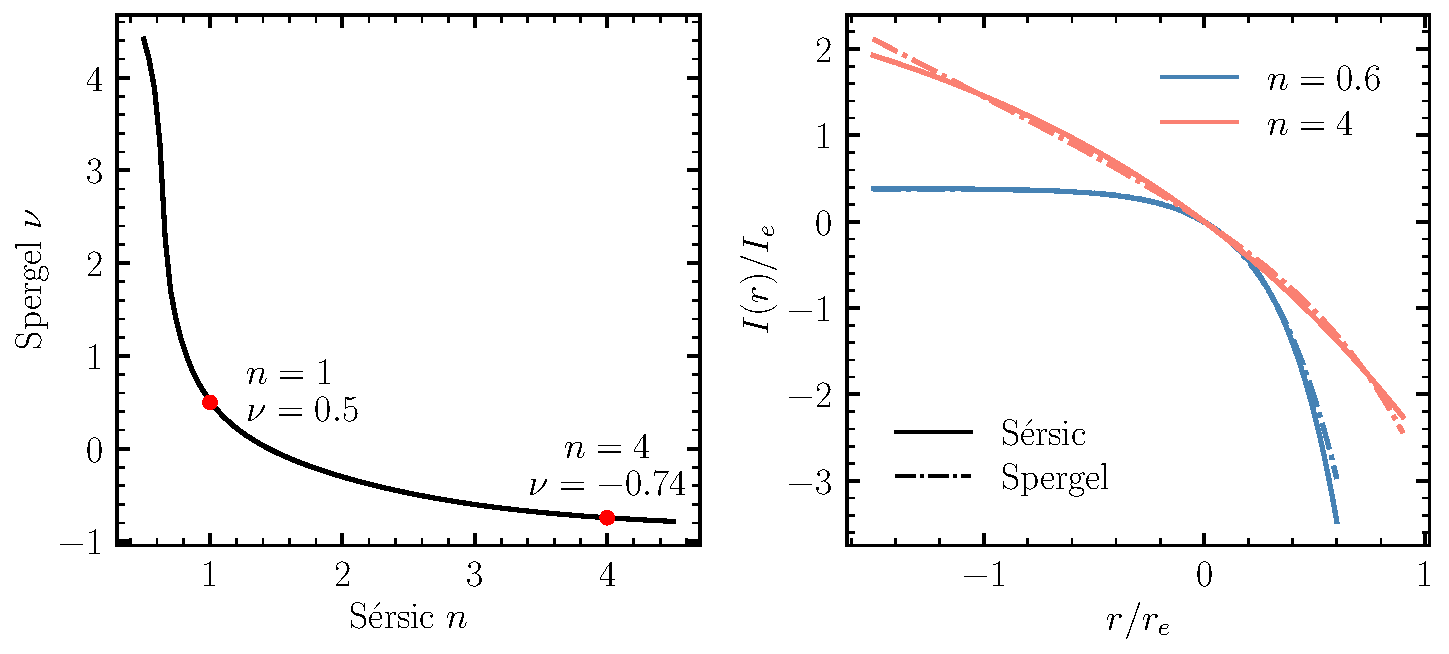
\includegraphics[width=0.75\linewidth]{spergel_sersic_calib.pdf}
	}
    \caption{The correspondence between the \sersic{} profile \eqref{eq:sersic} and the Spergel profile \eqref{eq:spergel}. We fit a Spergel profile to \sersic{} while fixing the total luminosity and half-light radius. The left panel shows the best-fit Spergel index $\nu$ as a function of \sersic{} index $n$. In the right panel, two \sersic{} profiles (solid) and their best-fit Spergel profiles (dash-dotted) are shown. Spergel profile approximates \sersic{} well for small \sersic{} indices.  
    }
    \label{fig:spgl_calib}
\end{figure*}

In this appendix, we demonstrate that the Spergel profile can approximate \sersic{} profile and profile a lookup table for the correspondence between \sersic{} index $n$ and Spergel index $\nu$.

The surface brightness of a \sersic{} profile follows \citep{Sersic1963,Graham2005}:
\begin{equation}\label{eq:sersic}
    I(r)=I_{\mathrm{e}} \exp \left\{-b_{n}\left[\left(\frac{r}{r_{\mathrm{e}}}\right)^{1 / n}-1\right]\right\},
\end{equation}
where $r_e$ is the half-light radius, $I_e$ is the surface brightness at $r=r_e$, $n$ is the \sersic{} index. The value of $b_n$ satisfies $\Gamma(2 n)=2 \gamma\left(2 n, b_{n}\right)$, where $\gamma(a, x)$ is the incomplete gamma function. According to \citet{Graham2005}, the total luminosity of a \sersic{} profile is given by 
\begin{equation}\label{eq:sersic_lum}
    L_0 = I_{e} r_{e}^{2}\, 2 \pi n\, e^{b_{n}} \left(b_{n}\right)^{-2 n} \Gamma(2 n).
\end{equation}
The Spergel profile is described in Section \ref{sec:modeling}. 

To study the correspondence between \sersic{} and Spergel profiles, we generate \sersic{} profiles with different \sersic{} indices, and try to fit Spergel profiles to \sersic{} ones. The \sersic{} index ranges from $n=0.5$ to $n=4.5$, and both profiles are normalized using $r_e$. For each \sersic{} profile, we calculate the total luminosity $L_0$ according to \eqref{eq:sersic_lum} and plug it into the Spergel profile \eqref{eq:spergel} as a fixed value. Therefore, only the Spergel index $\nu$ is allowed to vary during the fitting. The best-fit Spergel index $\nu$ as a function of \sersic{} index $n$ is shown in the left panel of Figure \ref{fig:spgl_calib}. As two examples, we show two \sersic{} profiles (solid) and their best-fit Spergel profiles (dash-dotted) in the right panel. A Spergel profile with $\nu=0.5$ is exactly an exponential profile with $n=1$. The de Vaucouleurs profile \citep{deVaucouleurs1948} with $n=4$ can be approximated by a Spergel profile with $\nu=-0.74$. 

As shown in Figure \ref{fig:spgl_calib}, a \sersic{} profile with small \sersic{} index ($0.5 < n < 1.5$) can be well-approximated by a Spergel profile, although the Spergel profile seems to be more extended than \sersic{} in the outskirts. For a \sersic{} profile with high \sersic{} index, the approximation gets worse at both small and large radii. Overall, the Spergel profile is a good approximation to \sersic{} from $n\approx 0.5$ to $n\approx 4.5$. It is well-known that the light profiles of low-mass galaxies are quite flat and can be described using \sersic{} profiles with $0.5 < n < 1.5$ \citep[e.g.,][]{vanDokkum2015,Lange2015,Greco2018,Zaritsky2021,ELVES-I}. It is thus reasonalbe to use Spergel profiles to model the LSBGs (Sec \ref{sec:modeling}) and enjoy its convenience in the Fourier space. 



% \section{Measurement Error}\label{ap:meas_error}

% We characterize the quality of the Spergel modeling by injecting mock \sersic{} galaxies into the cutout and compare the recovered properties with the truth, as shown in Appendix \ref{ap:meas_error}. Overall speaking, the measurement agrees with the truth quite well. However, the size and the total flux of galaxies below $\overline{\mu}_{\rm eff} (g) > 27$ is under-estiamted. We also characterize the bias and the scatter in measurement as a function of size and surface brightness. We apply the bias correction to the measurement of LSBGs, and incorporate the measurement error into the science figures. 

% vdB 16 doesn't consider whether GALFIT gives the corrrect $R_e$, when deriving the completeness (recovered fraction)

% Remember to ref SMUDGES papers here.


\section{UDG and UPG Catalogs}
\onecolumngrid 

\begin{table}
\caption{UDG (UPG) catalog description} 
\label{tab:catalog}
\begin{center}
\begin{tabular}{l l l}
\hline\hline
% \multicolumn{3}{c}{Table: LSBGs (781 rows)}                 \\
% \hline
Column Name      & Unit    & Description                    \\
\hline
ID                       &         & Unique LSBG ID \\
ra                       & deg     & Right ascension (J2000) \\
dec                      & deg     & Declination (J2000) \\
$r_e$         & arcsec  & Circularized effective radius  \\
$\sigma(r_e)$ & arcsec  & Uncertainty of $r_e$ \\
$\overline{\mu}_{\mathrm{eff}}(g)$               & $\sbunit$ & $g$-band average surface brightness within $r_e$ \\
$\sigma(\overline{\mu}_{\mathrm{eff}}(g))$       & $\sbunit$ & Uncertainty of $\overline{\mu}_{\mathrm{eff}}(g)$           \\
% $\overline{\mu}_{\mathrm{eff}}(r)$               & $\sbunit$ & $r$-band average surface brightness within $r_e$ \\
% $\sigma(\overline{\mu}_{\mathrm{eff}}(r))$       & $\sbunit$ & Uncertainty of $\overline{\mu}_{\mathrm{eff}}(r)$           \\
% $\overline{\mu}_{\mathrm{eff}}(i)$               & $\sbunit$ & $i$-band average surface brightness within $r_e$ \\
% $\sigma(\overline{\mu}_{\mathrm{eff}}(i))$       & $\sbunit$ & Uncertainty of $\overline{\mu}_{\mathrm{eff}}(i)$           \\
$m_g$                    & mag     & $g$-band apparent magnitude     \\
$\sigma(m_g)$            & mag     & Uncertainty of $m_g$            \\
% $m_r$                    & mag     & $r$-band apparent magnitude     \\
% $\sigma(m_r)$            & mag     & Uncertainty of $m_r$            \\
% $m_i$                    & mag     & $i$-band apparent magnitude     \\
% $\sigma(m_i)$            & mag     & Uncertainty of $m_i$            \\
$g-r$                    & mag     & $g-r$ color                     \\
$\sigma(g-r)$            & mag     & Uncertainty of $g-r$ color      \\
$g-i$                    & mag     & $g-i$ color                     \\
$\sigma(g-i)$            & mag     & Uncertainty of $g-i$ color      \\
$\nu$                    &         & Spergel index              \\
$\varepsilon$            &         & Ellipticity                     \\
$A_g$                    & mag     & $g$-band Galactic extinction \\
$A_r$                    & mag     & $r$-band Galactic extinction \\
$A_i$                    & mag     & $i$-band Galactic extinction \\
$\log\ M_\star$ & $M_\odot$ & Stellar mass of UDG (UPG) \\
comp & & Completeness \\
weight & & Color-dependent weight (see Section \ref{sec:bkg}) \\
host\_name & & Name of the host galaxy \\
host\_ra & & Right ascension (J2000) of the host galaxy \\
host\_dec & & Declination (J2000) of the host galaxy \\
host\_log\_m\_star & $M_\odot$ & Host stellar mass\\
host\_r\_vir & kpc & Virial radius of the host galaxy \\
host\_g\_i & mag & $g-i$ color of the host galaxy \\
host\_z &  & Redshift of the Host galaxy \\
sep\_to\_host & deg & Angular separation between the host and UDG (UPG)\\
\hline\hline
\end{tabular}
\end{center}
\tablecomments{
These tables are published in their entirety in machine-readable format.
Magnitudes are on the AB system and have been corrected for measurement biases and Galactic
extinction. The information of the host galaxies is from NASA-Sloan Atlas. We provide Galactic extinction corrections, which are derived from
the \citet{Schlafly2011} recalibration of the \citet{SFD1998} dust maps. 
}
\end{table}

Also add external link for fake UDG catalog, etc. 


\end{CJK*}
\end{document}